\chapter{概要设计}

本章主要介绍本系统的概要设计，重点针对AI多任务场景下系统适配性差、调度决策太依赖人工以及资源互斥识别难这三大核心子问题，给出了层级化的架构设计思路。整个系统分为API接入层、任务调度层和任务执行层：API层和执行层主要负责解决“适配”问题，通过建立大模型任务参数画像，实现了对AI异构数据的自动纠错与类型推断；任务调度层则是系统的“指挥中枢”，通过引入环境感知的自动化决策引擎和资源互斥智能分析算法，让任务能脱离人工干预自动下发，并有效解决了资源抢占导致的串行效率低下难题。通过这三层架构的紧密协作，系统完成了由传统排队模式向智能化、高并发调度的转型，为后续的功能实现与工业推广打下了坚实的架构基础。

\section{AI多任务资源调度系统基本原则}

为确保系统能够有效应对AI大模型任务的高算力需求与复杂数据特征，本系统在架构设计阶段遵循以下核心原则：

\begin{enumerate}
	\item 异构参数适配与数据鲁棒性原则。针对AI大模型任务参数格式多样且极易出错的特征，系统需在数据接入端强化Schema层级的深度校验。设计应具备对全角/半角符号、非法字符及数据类型的自动纠偏逻辑，确保异构参数在分布式传递过程中的语义一致性，从源头提升系统的容错能力与数据处理门槛。
    \item 环境感知与决策自主化原则。针对任务调度过度依赖人工干预的现状，系统应具备对计算集群负载、网络状态及运营策略的实时感知能力。通过构建基于逻辑引擎的自主决策机制，将传统的“人工触发”转化为“策略驱动”，实现调度流程的自动化闭环，以提升系统在高动态环境下的响应效能。
    \item 临界资源隔离与并发安全原则。算力资源的精准治理是系统的核心目标。设计必须建立细粒度的“资源-任务”映射关系，通过互斥检测算法识别任务间的算力冲突（如GPU显存抢占）。系统应支持在保障资源独占安全的前提下，通过智能并发策略取代传统串行模式，最大化集群吞吐率并降低算力空耗。
    \item 架构分层解耦与弹性扩展原则。系统应遵循模块化设计思想，将API接入、任务调度与分布式执行进行逻辑解耦。各层级间通过标准化协议通信，确保系统具备良好的水平扩展能力，以便在计算负载激增时，能够通过动态增加执行节点（Worker）完成算力的线性扩容。
    \item 细粒度权限管控与合规性原则。鉴于AI算力资源的昂贵性与数据的敏感性，系统必须构建严密的鉴权体系。基于“任务组”实现多租户隔离与访问控制策略（RBAC），严格限制非授权用户对临界资源的占用与调度指令的干预，确保生产环境下的资源分配安全性与审计合规性。
\end{enumerate}
 
\section{AI多任务资源调度系统整体结构}

\begin{figure}[ht]
    \centering
    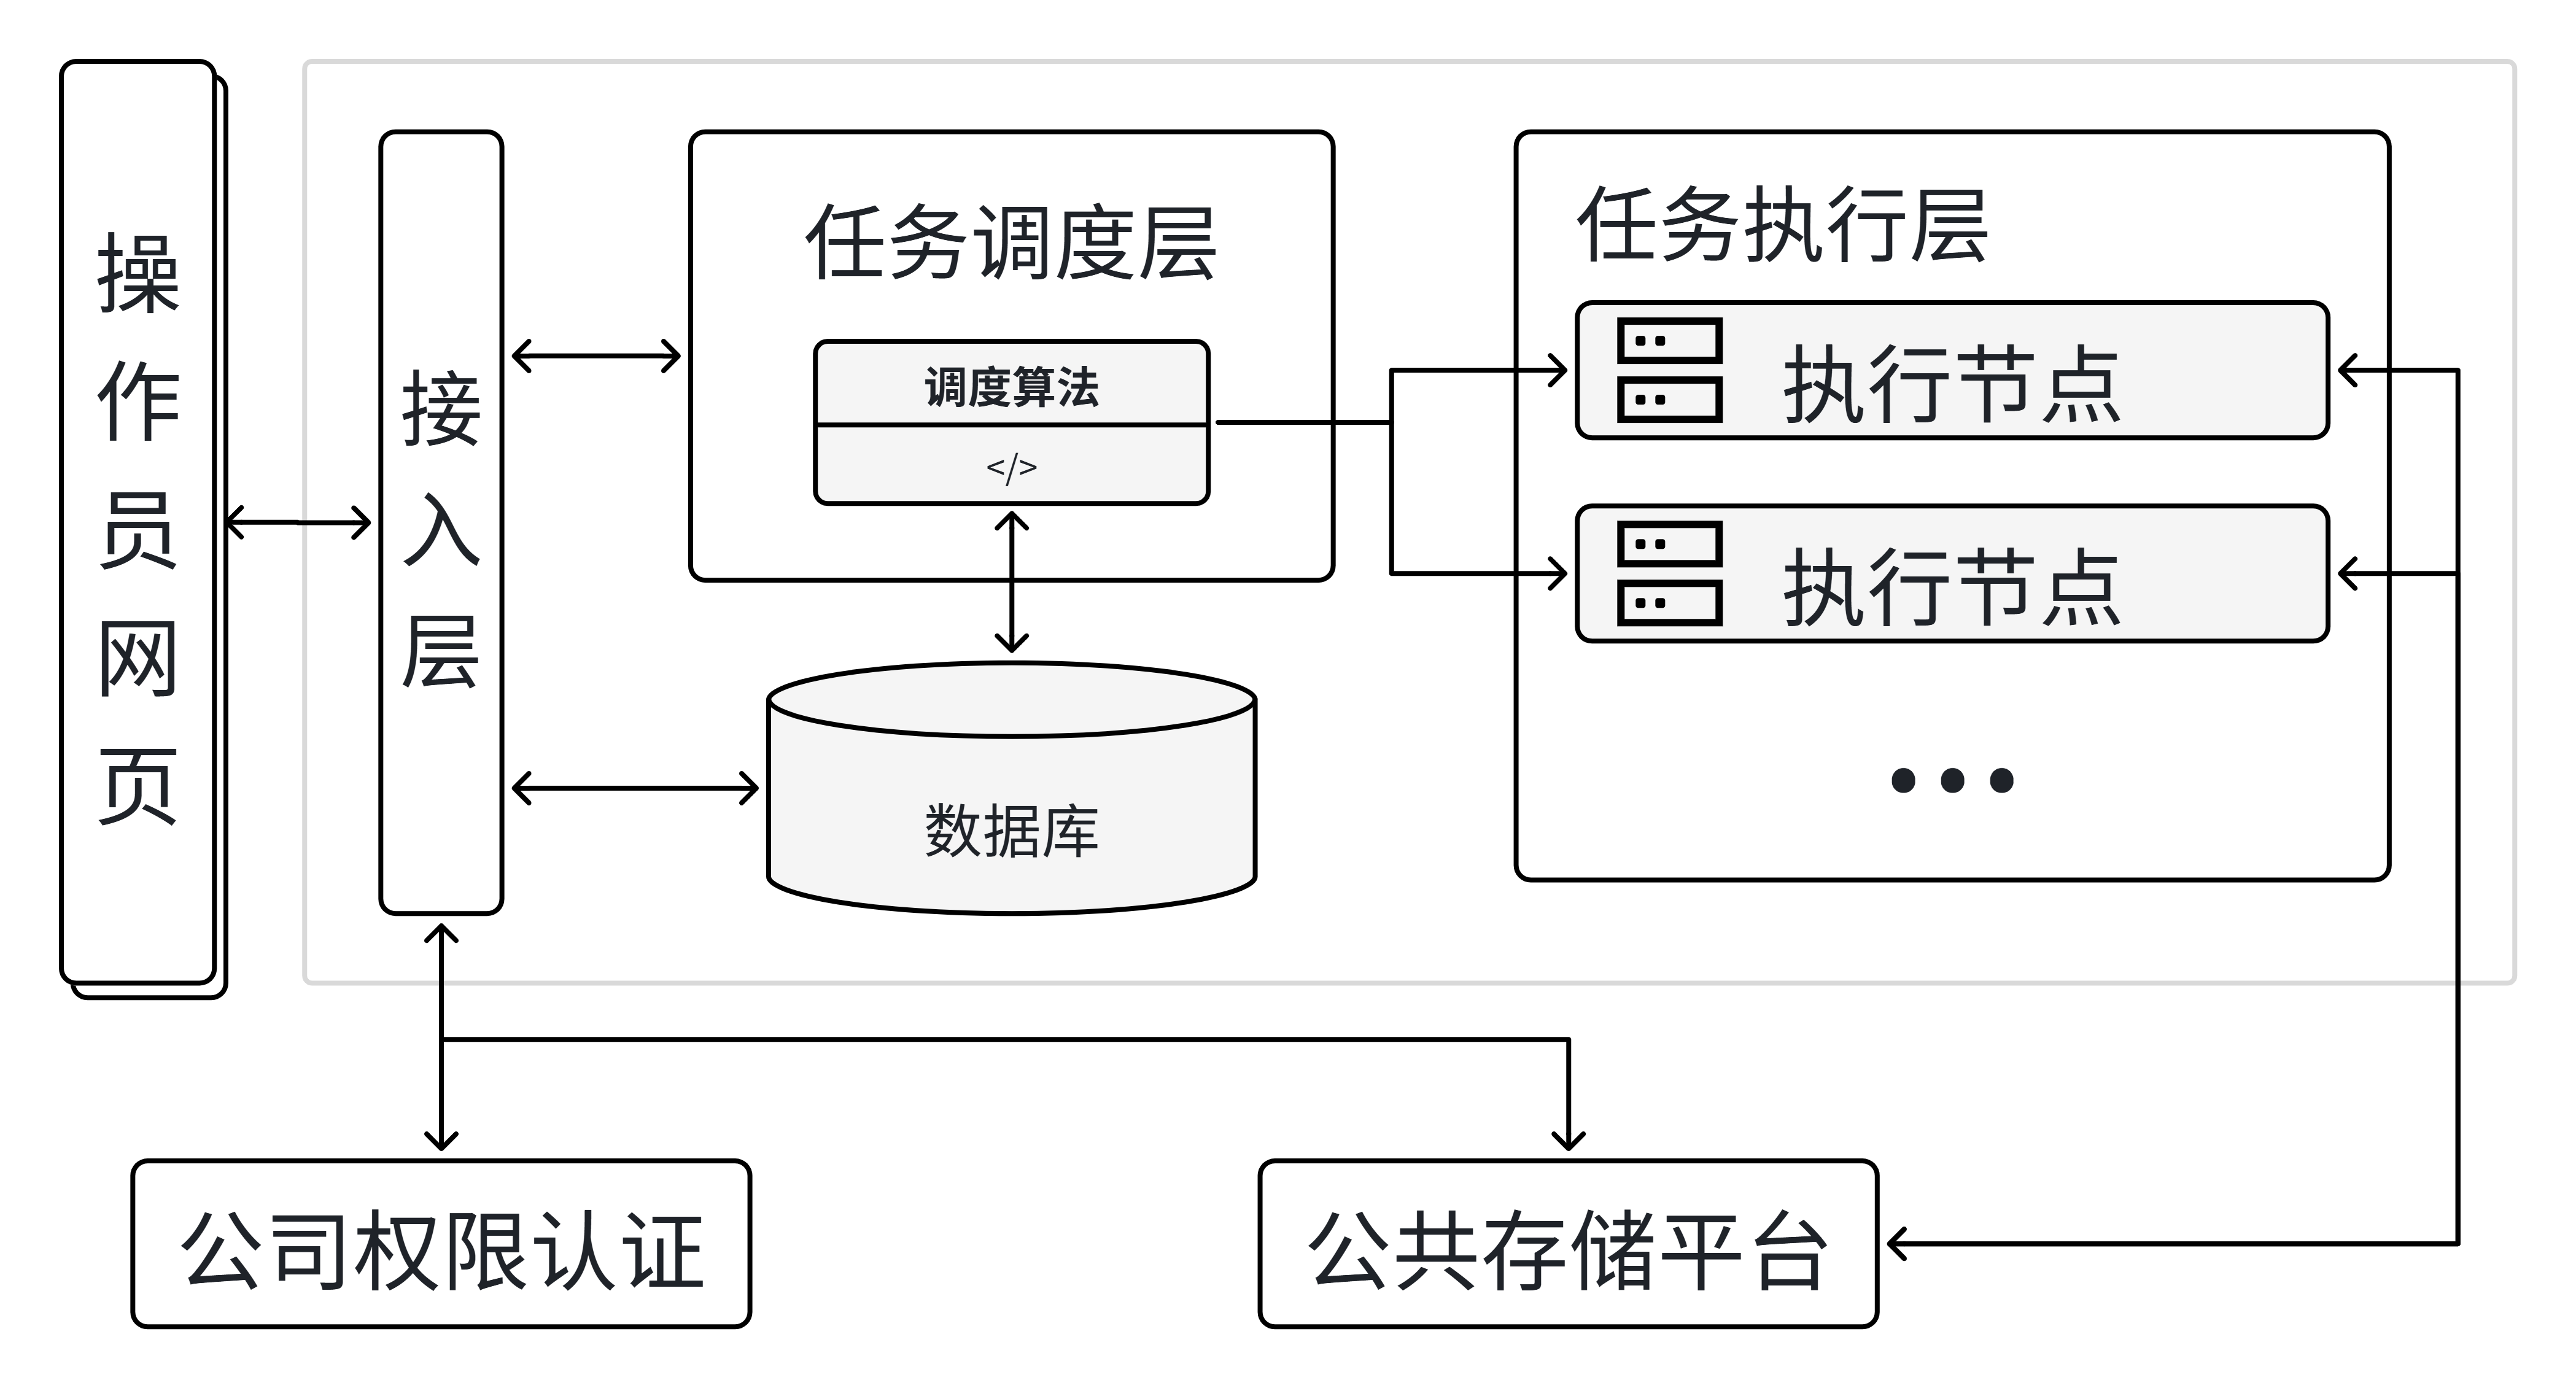
\includegraphics[width=\linewidth]{figures/4/系统整体架构.png}
    \caption{系统整体架构图}
    \label{fig:enter-label}
\end{figure}

本系统整体结构如图4.1所示。为有效应对前文提出的三大核心挑战，系统采用分层解耦的软件架构设计，将复杂的调度逻辑划分为三个功能层级，各层间通过标准化接口进行数据交互，确保系统具备高内效能与良好的扩展性。简要介绍如下：

\begin{enumerate}
    \item API接入层。该层作为系统与外部交互的唯一门户，主要负责请求拦截、身份核验与初步数据治理。针对子问题一，本层重点设计了异构数据自动纠偏机制。在HTTP过滤层完成公司级鉴权后，系统会对输入的Prompt模板及AI超参数进行Schema校验，自动修正字符格式偏差与类型冲突，从源头保障任务数据的纯净度，解决现有系统适配性欠佳的问题。
    \item 任务调度层。该层是系统的决策大脑，由任务池、自动化决策引擎、同步模块及容错恢复模块组成。针对子问题二，调度层通过逻辑引擎实时感知系统负载，自主判定任务执行条件，消除了对人工触发的依赖；针对子问题三，该层引入了临界资源互斥分析算法，通过动态扫描资源占用表，精准识别任务间的算力冲突，将传统的保守串行调度优化为智能并发调度，显著提升了算力利用率。
    \item 任务执行层。该层由分布式的任务执行器（Worker）构成，直接对接公司存储服务与GPU算力资源平台。其内部设有参数本地化处理、任务执行监控及结果上报模块。该层负责接收调度层下发的指令，执行具体的AI模型推理或测试任务。通过细粒度的异常捕获机制，该层能实时反馈节点运行状态，配合调度层的容灾逻辑，确保在异构环境下任务执行的鲁棒性与一致性。
\end{enumerate}

\section{API接入层概要设计}

API接入层承担系统的安全准入与数据治理职能。在承载高并发请求的基础上，该层通过身份鉴权与参数标准化预处理构建合规屏障。本层重点引入参数画像校验与自动纠偏逻辑，在入口处即时拦截并修复人工录入偏差，确保调度指令的高度一致性与鲁棒性，从源头解决AI异构数据的适配难题。

\subsection{权限鉴定模块}

鉴权模块分为两部分：身份认证、权限判定。身份认证功能以一个Python函数的形式注册成为了FastAPI框架的一个中间件。中间件是一种位于操作系统和应用程序之间的软件层，用于解决不同系统之间的数据格式转换、通信协议适配等问题\cite{9}。身份认证功能的时序如下图4.2所示：

\begin{figure}[htbp]
    \centering
    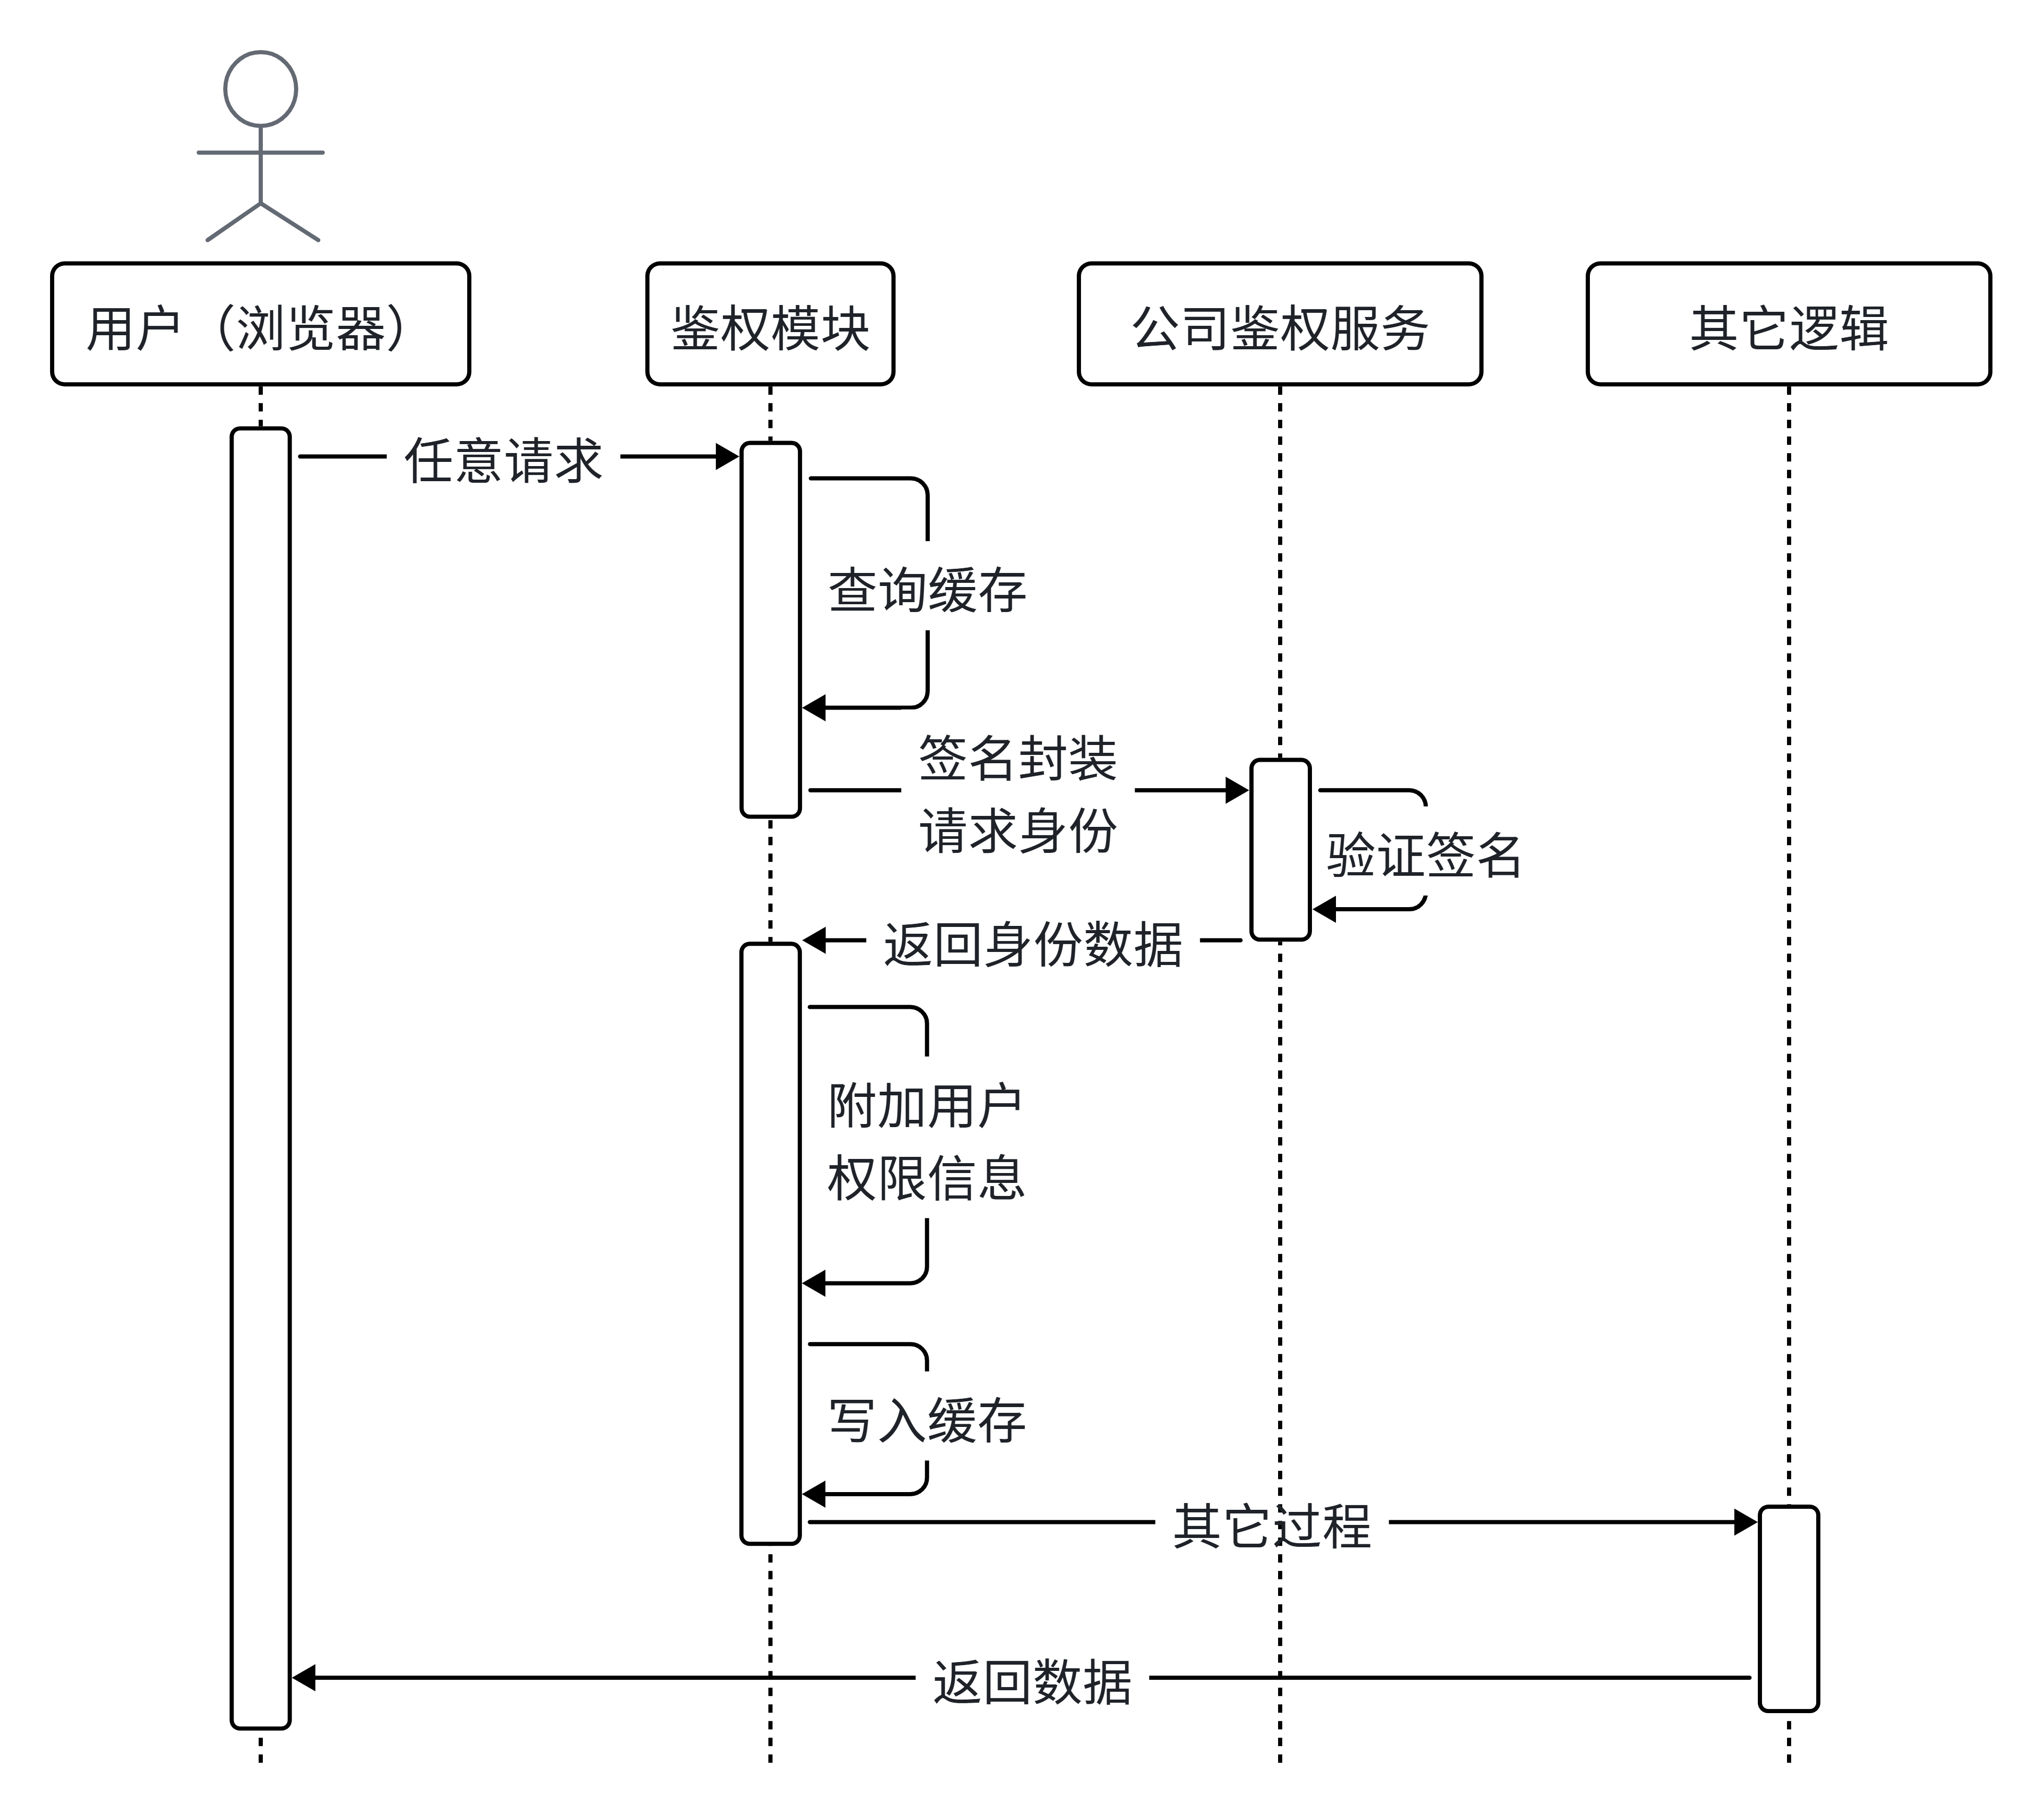
\includegraphics[width=\linewidth]{figures/4/身份认证流程.png}
    \caption{身份认证时序图}
    \label{fig:enter-label}
\end{figure}

首先，系统接收外部传入的请求，进入处理环节后，第一步是解析请求里包含的身份相关参数，这些参数是后续身份验证的基础；接着，利用解析出的参数向公司认证服务器发起请求，借助认证服务器的校验能力，获取到关于请求来源的准确身份信息；最后，把获取到的身份信息整合到原始请求的数据内容里，使后续业务处理流程能基于包含完整身份信息的请求开展，保障业务逻辑中对身份维度的需求，规范且有序地完成从请求接入到身份信息准备就绪的过程。

权限判定模块则是用于判断某个用户是否有权限操作本任务组。权限判定需要基于身份认证提供的用户信息，所以安排在身份认证之后。权限判定以一个独立部署的微服务的形式服务于本系统，有自己的前后端，结构如图4.3所示：

\begin{figure}[htbp]
    \centering
    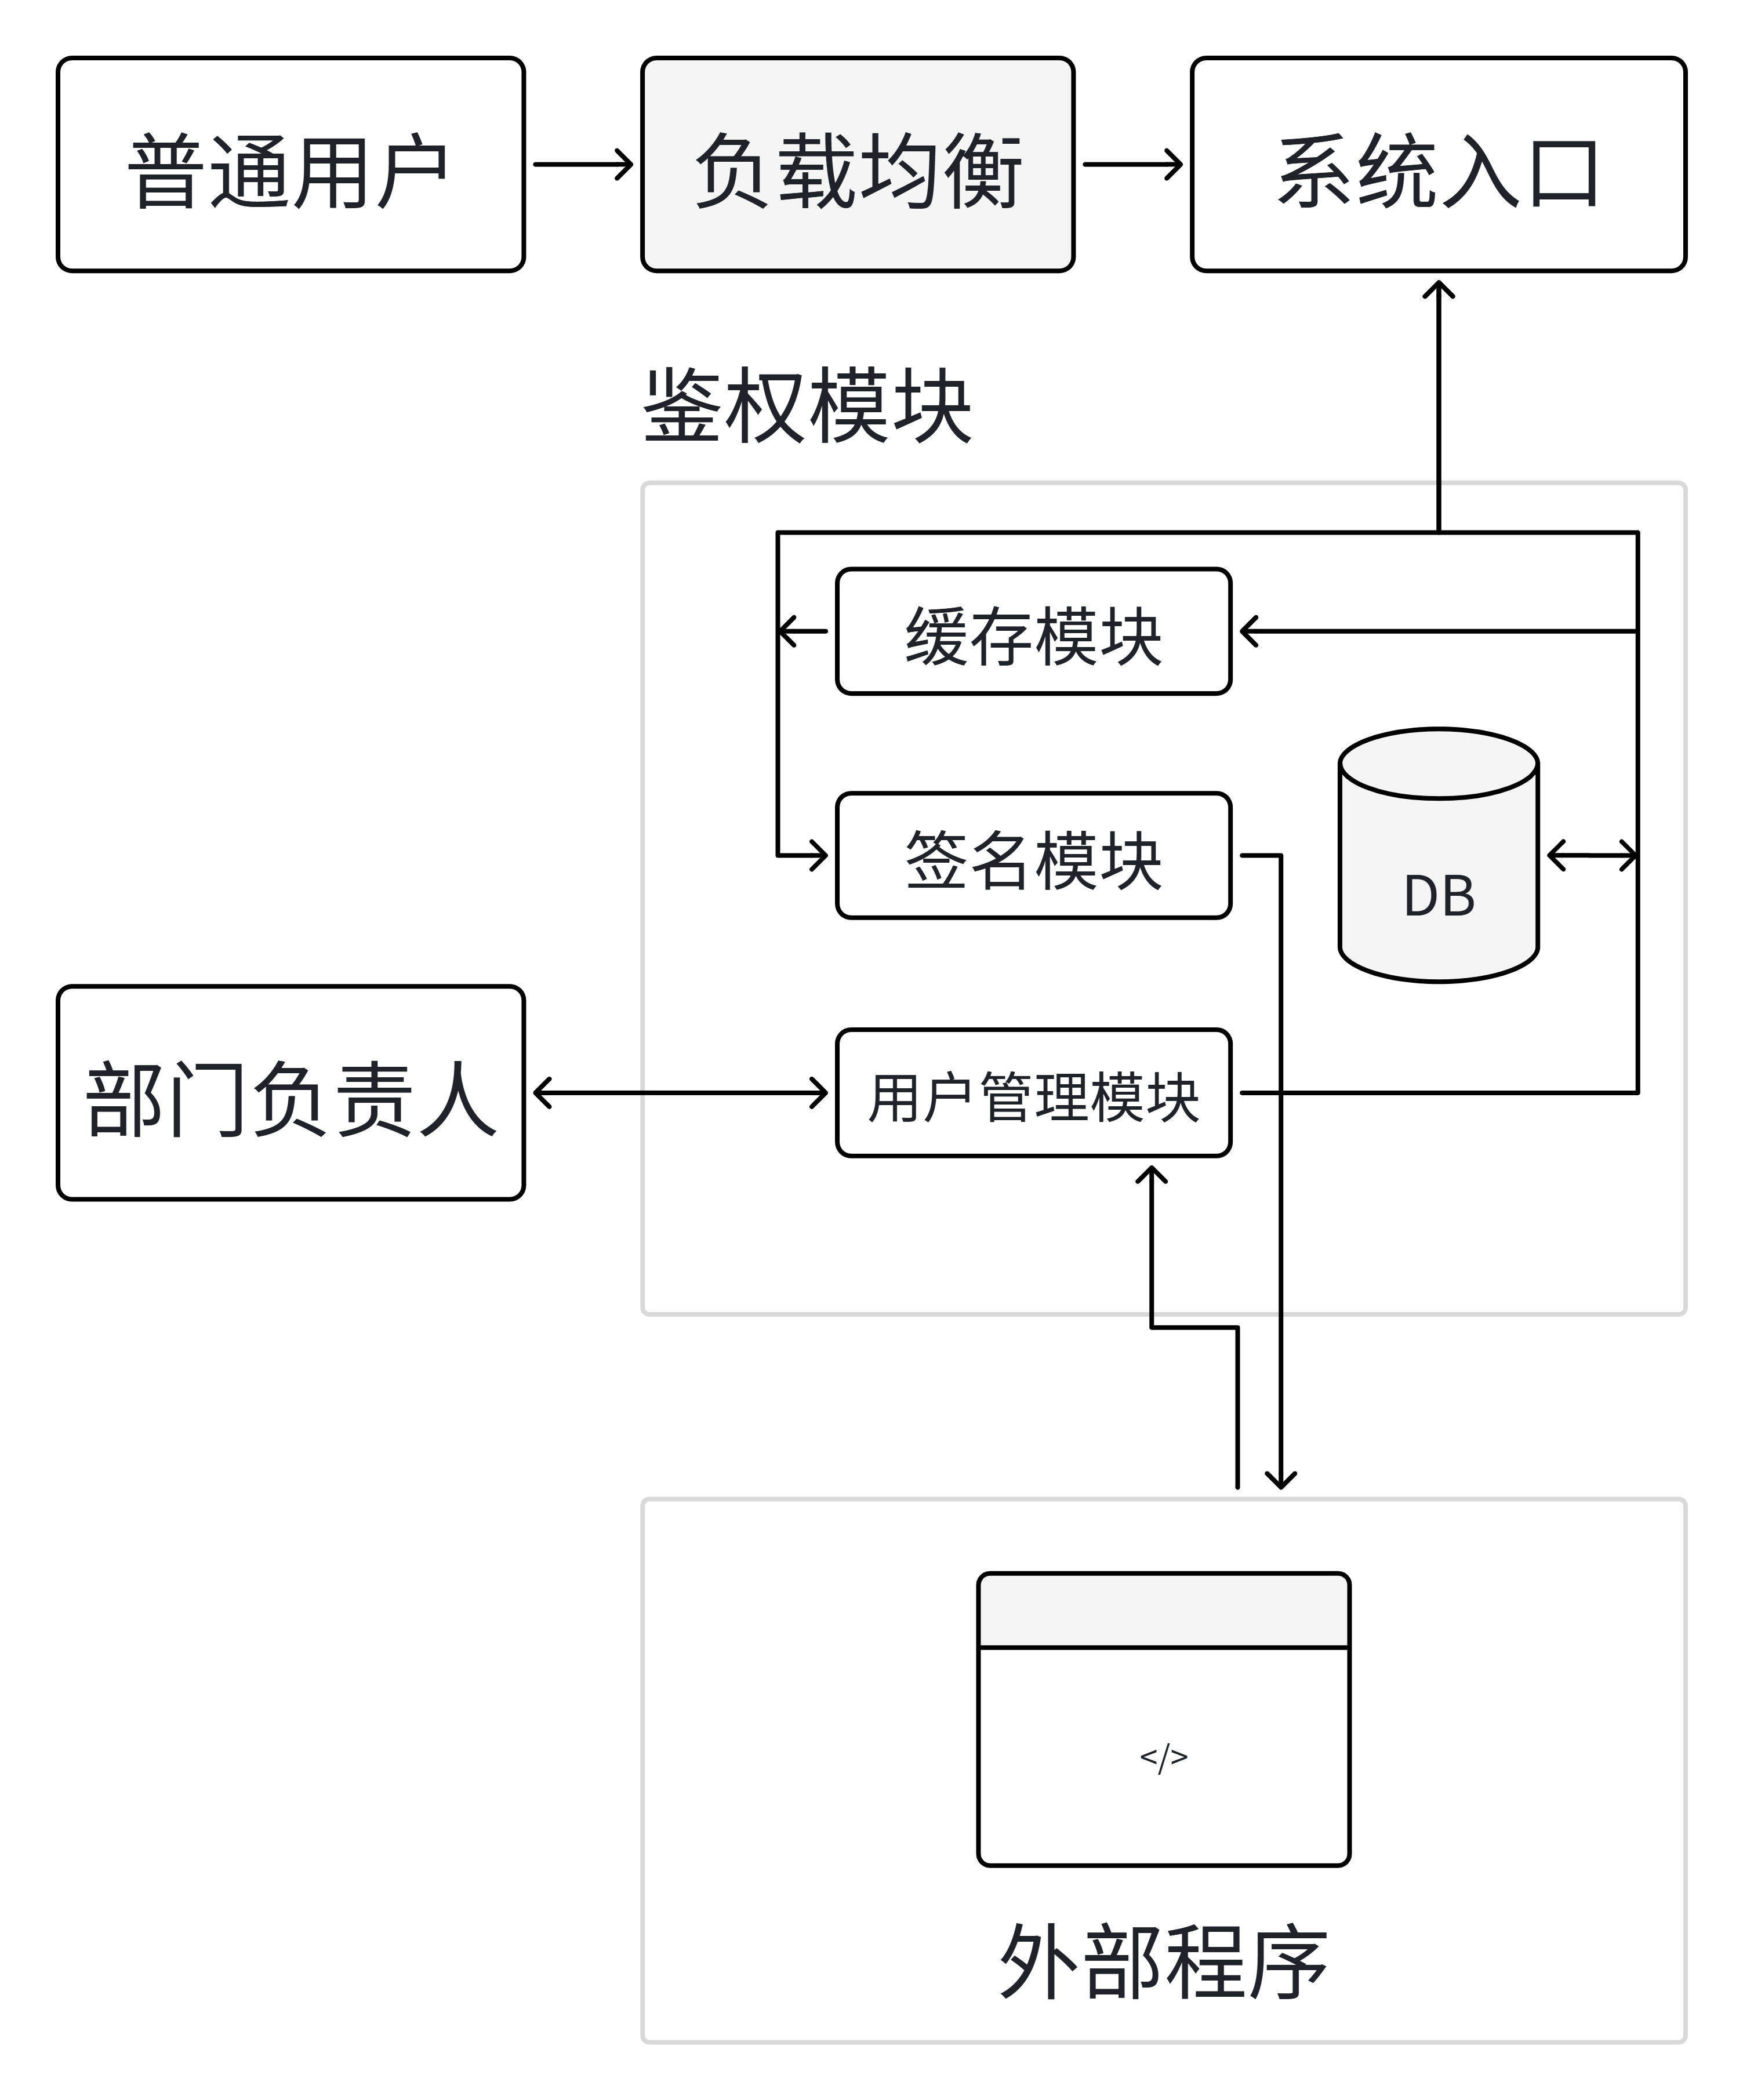
\includegraphics[width=0.6\linewidth]{figures/4/鉴权服务架构图.png}
    \caption{鉴权服务架构图}
    \label{fig:enter-label}
\end{figure}

部门负责人通过网页操作触发鉴权系统Web端，或由其他服务发起，均以HTTP请求形式传递至鉴权服务器 。鉴权服务器先经 “HTTP请求处理” 模块接收请求，再联动 “用户管理模块”与“签名验证模块”开展身份校验逻辑，过程中通过TCP协议与数据库服务器的PostgreSQL交互，查询、验证用户数据，以此实现对各类请求的鉴权管理，保障系统访问安全与权限合规。

\subsection{数据校验模块}

Pydantic是一个用Python编写的数据验证和设置管理库，基于Python的类型注解来进行数据验证等操作，在数据处理和API开发等场景中被广泛应用。本系统采用Python生态内的Pydantic库来对请求数据结构进行初步的校验。在本系统的数据结构定义层，设有一个特定目录，专门用于存放HTTP请求数据结构的定义内容。对于每个请求，均有相应的类来记录请求数据格式与响应数据格式。此外，还存在一些通用的基本结构，这些结构为所有请求和响应提供基础的数据表单。本系统以FastAPI中间件的形式，将Pydantic注册进来，以此实现无感的数据类型校验。

\subsection{业务模块}

本系统构建了以任务、统计、附件、任务组及用户为核心的五类业务API，旨在实现AI任务全生命周期的精细化管理。各API模块通过双向交互保障数据库的一致性，并深度联动鉴权模块实现细粒度的操作授权。

在底层调度逻辑上，系统利用FastAPI异步框架配合定时任务入池，依托Redis作为消息中间件（Broker）驱动Celery分布式架构。这一设计为自动化决策判断与资源互斥智能分析提供了高性能的任务分发底座。任务经由Celery Worker执行后，其进度与结果通过反向流转机制实时更新至数据库并反馈至操作面板，从而形成了从指令下发到状态回收的完整自动化业务闭环。

\section{任务调度层概要设计}

本小节着重描述和任务调度、逻辑计算相关的设计。平台收到来自前端的任务请求时，会先生成一个任务表单，加进任务池中。任务池本质上是数据库中的一个表，每个任务有自己的参数和状态。处于“等待”状态的任务会被调度模块定期检查，符合任务执行条件（任务可用、资源不冲突）时，就会加入任务队列中。同步模块负责监控任务执行程序，定期拉取处于“执行中”任务的状态，将状态写入任务池（数据库），显示到网页里，供操作员参考。

\subsection{任务可用性检测机制}

“任务可用性”是对AI任务在特定时空背景下执行合规性的多维度评估。针对调度决策过度依赖人工经验的痛点，本系统构建了基于环境感知策略驱动的逻辑引擎，旨在实现调度流程的去人工化。该机制的核心在于业务策略与调度逻辑的深度解耦。系统通过以下流程实现自动化准入控制：

\begin{enumerate}
    \item 策略配置与解析：管理员通过配置平台动态维护基于JSON格式的策略描述文件。该文件定义了涵盖任务优先级、实时系统负载阈值、特定时间窗口限制及业务场景约束等关键指标。
    \item 动态映射：系统实时监测并读取配置平台下发的JSON格式策略文件。在解析过程中，引擎并非简单的字符串匹配，而是将JSON格式的抽象策略描述精准映射为系统内部可直接调用的可计算逻辑算子。每一个配置项都会被实例化为一个具备逻辑判定能力的算子对象，这些对象按照预设的逻辑拓扑结构进行组织，最终在内存中构建出一套高性能的动态规则库。
    \item 实时准入判定：当任务处于“待调度”状态并进入决策周期时，逻辑引擎会自动触发判定流程。通过规则引擎内部的布尔演算，系统能够自主、快速地判定该任务当前是否具备启动条件。若判定结果为真，则立即下发执行指令；若环境指标触碰“熔断”红线，任务将自动保持在等待队列中。
    \item 调度闭环管理：对于判定为不满足执行条件的任务，系统将其自动置入高可靠等待队列。调度器将持续轮询环境状态，直至满足策略要求后自动触发执行。
\end{enumerate}

通过这种“策略驱动”的自动化机制，系统有效消除了传统调度模式中对人工干预的依赖，在保障系统运行平稳的同时，显著提升了多任务并发场景下的决策效率。

\begin{figure}[htbp]
    \centering
    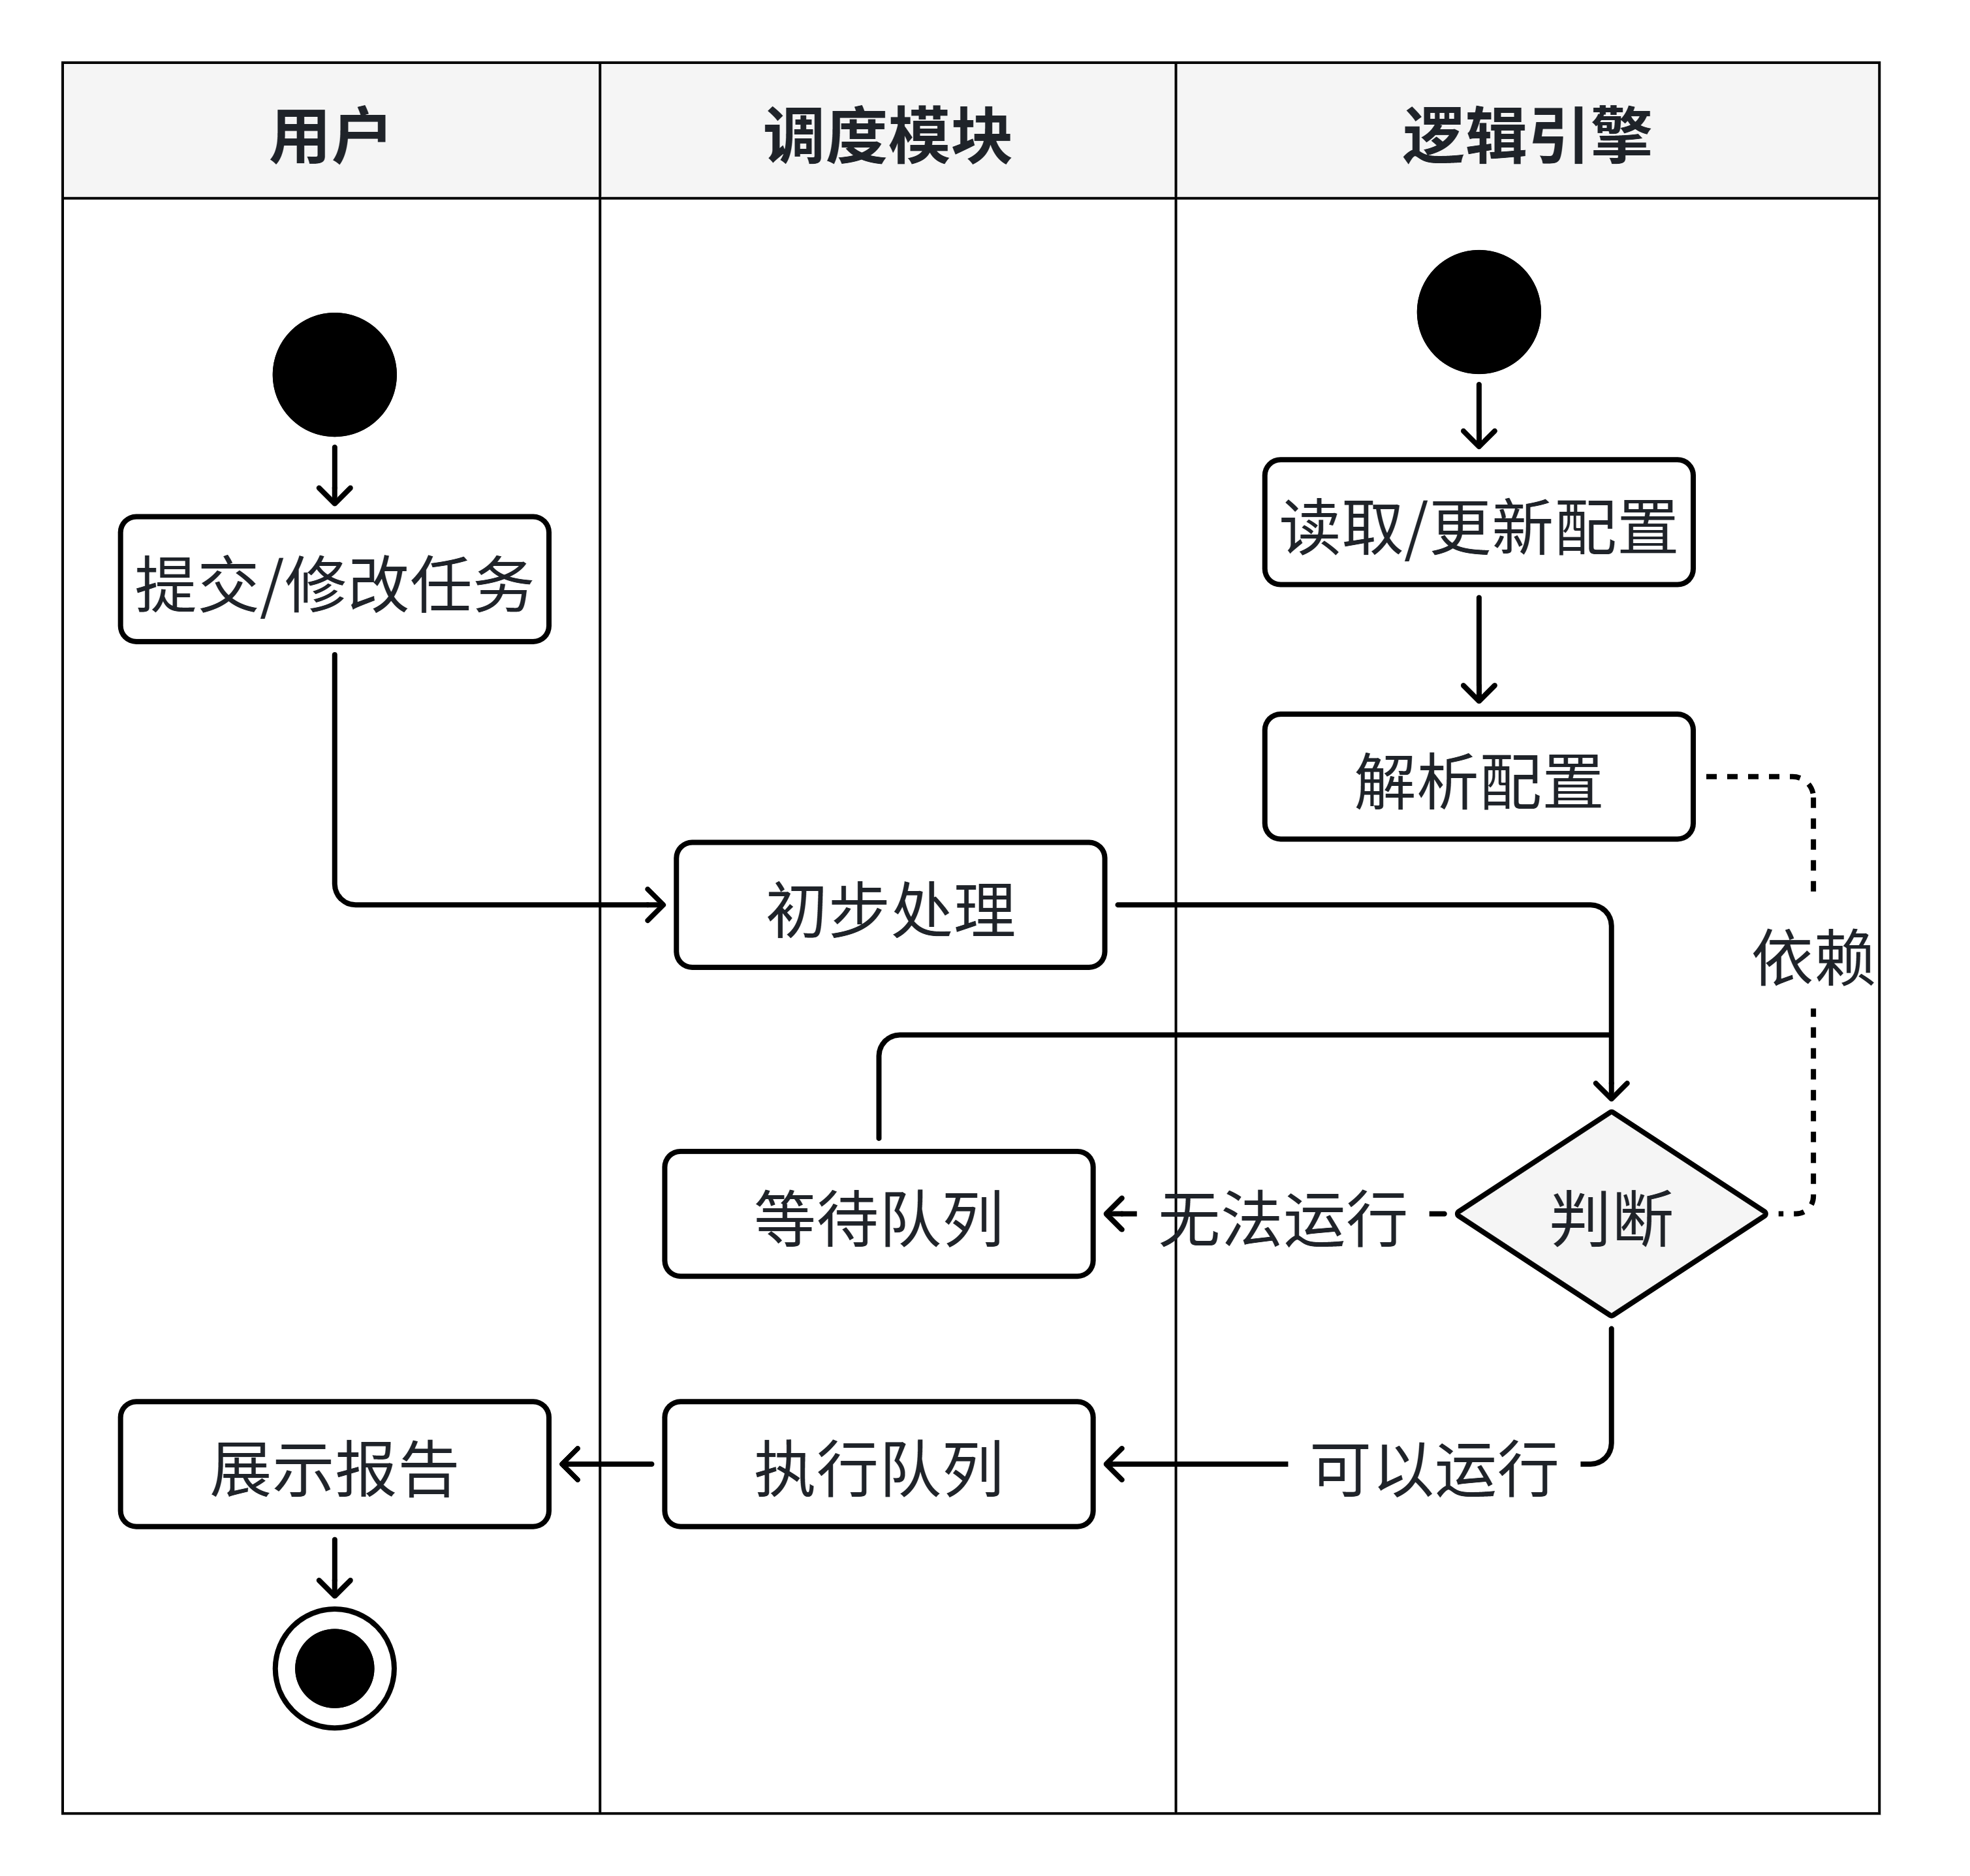
\includegraphics[width=0.8\linewidth]{figures/4/任务可用性判断流程图.png}
    \caption{任务可用性判断泳道图}
    \label{fig:enter-label}
\end{figure}

任务可用性判断流程如图4.4所示。当用户通过操作面板提交或修改任务请求后，调度模块首先执行基础的参数预处理，随后将其透传至逻辑引擎进行准入判定。逻辑引擎基于预解析的规则库，结合任务特征与当前系统环境约束，自主决定任务的执行时机：若判定为“无法运行”，任务将进入等待队列挂起，直至满足条件后被自动唤醒；若满足条件，则分发至执行队列并向用户展示反馈报告。该流程实现了从“人工干预”向“引擎自决”的转变，是提升调度自动化水平的关键环。

\begin{figure}[htbp]
    \centering
    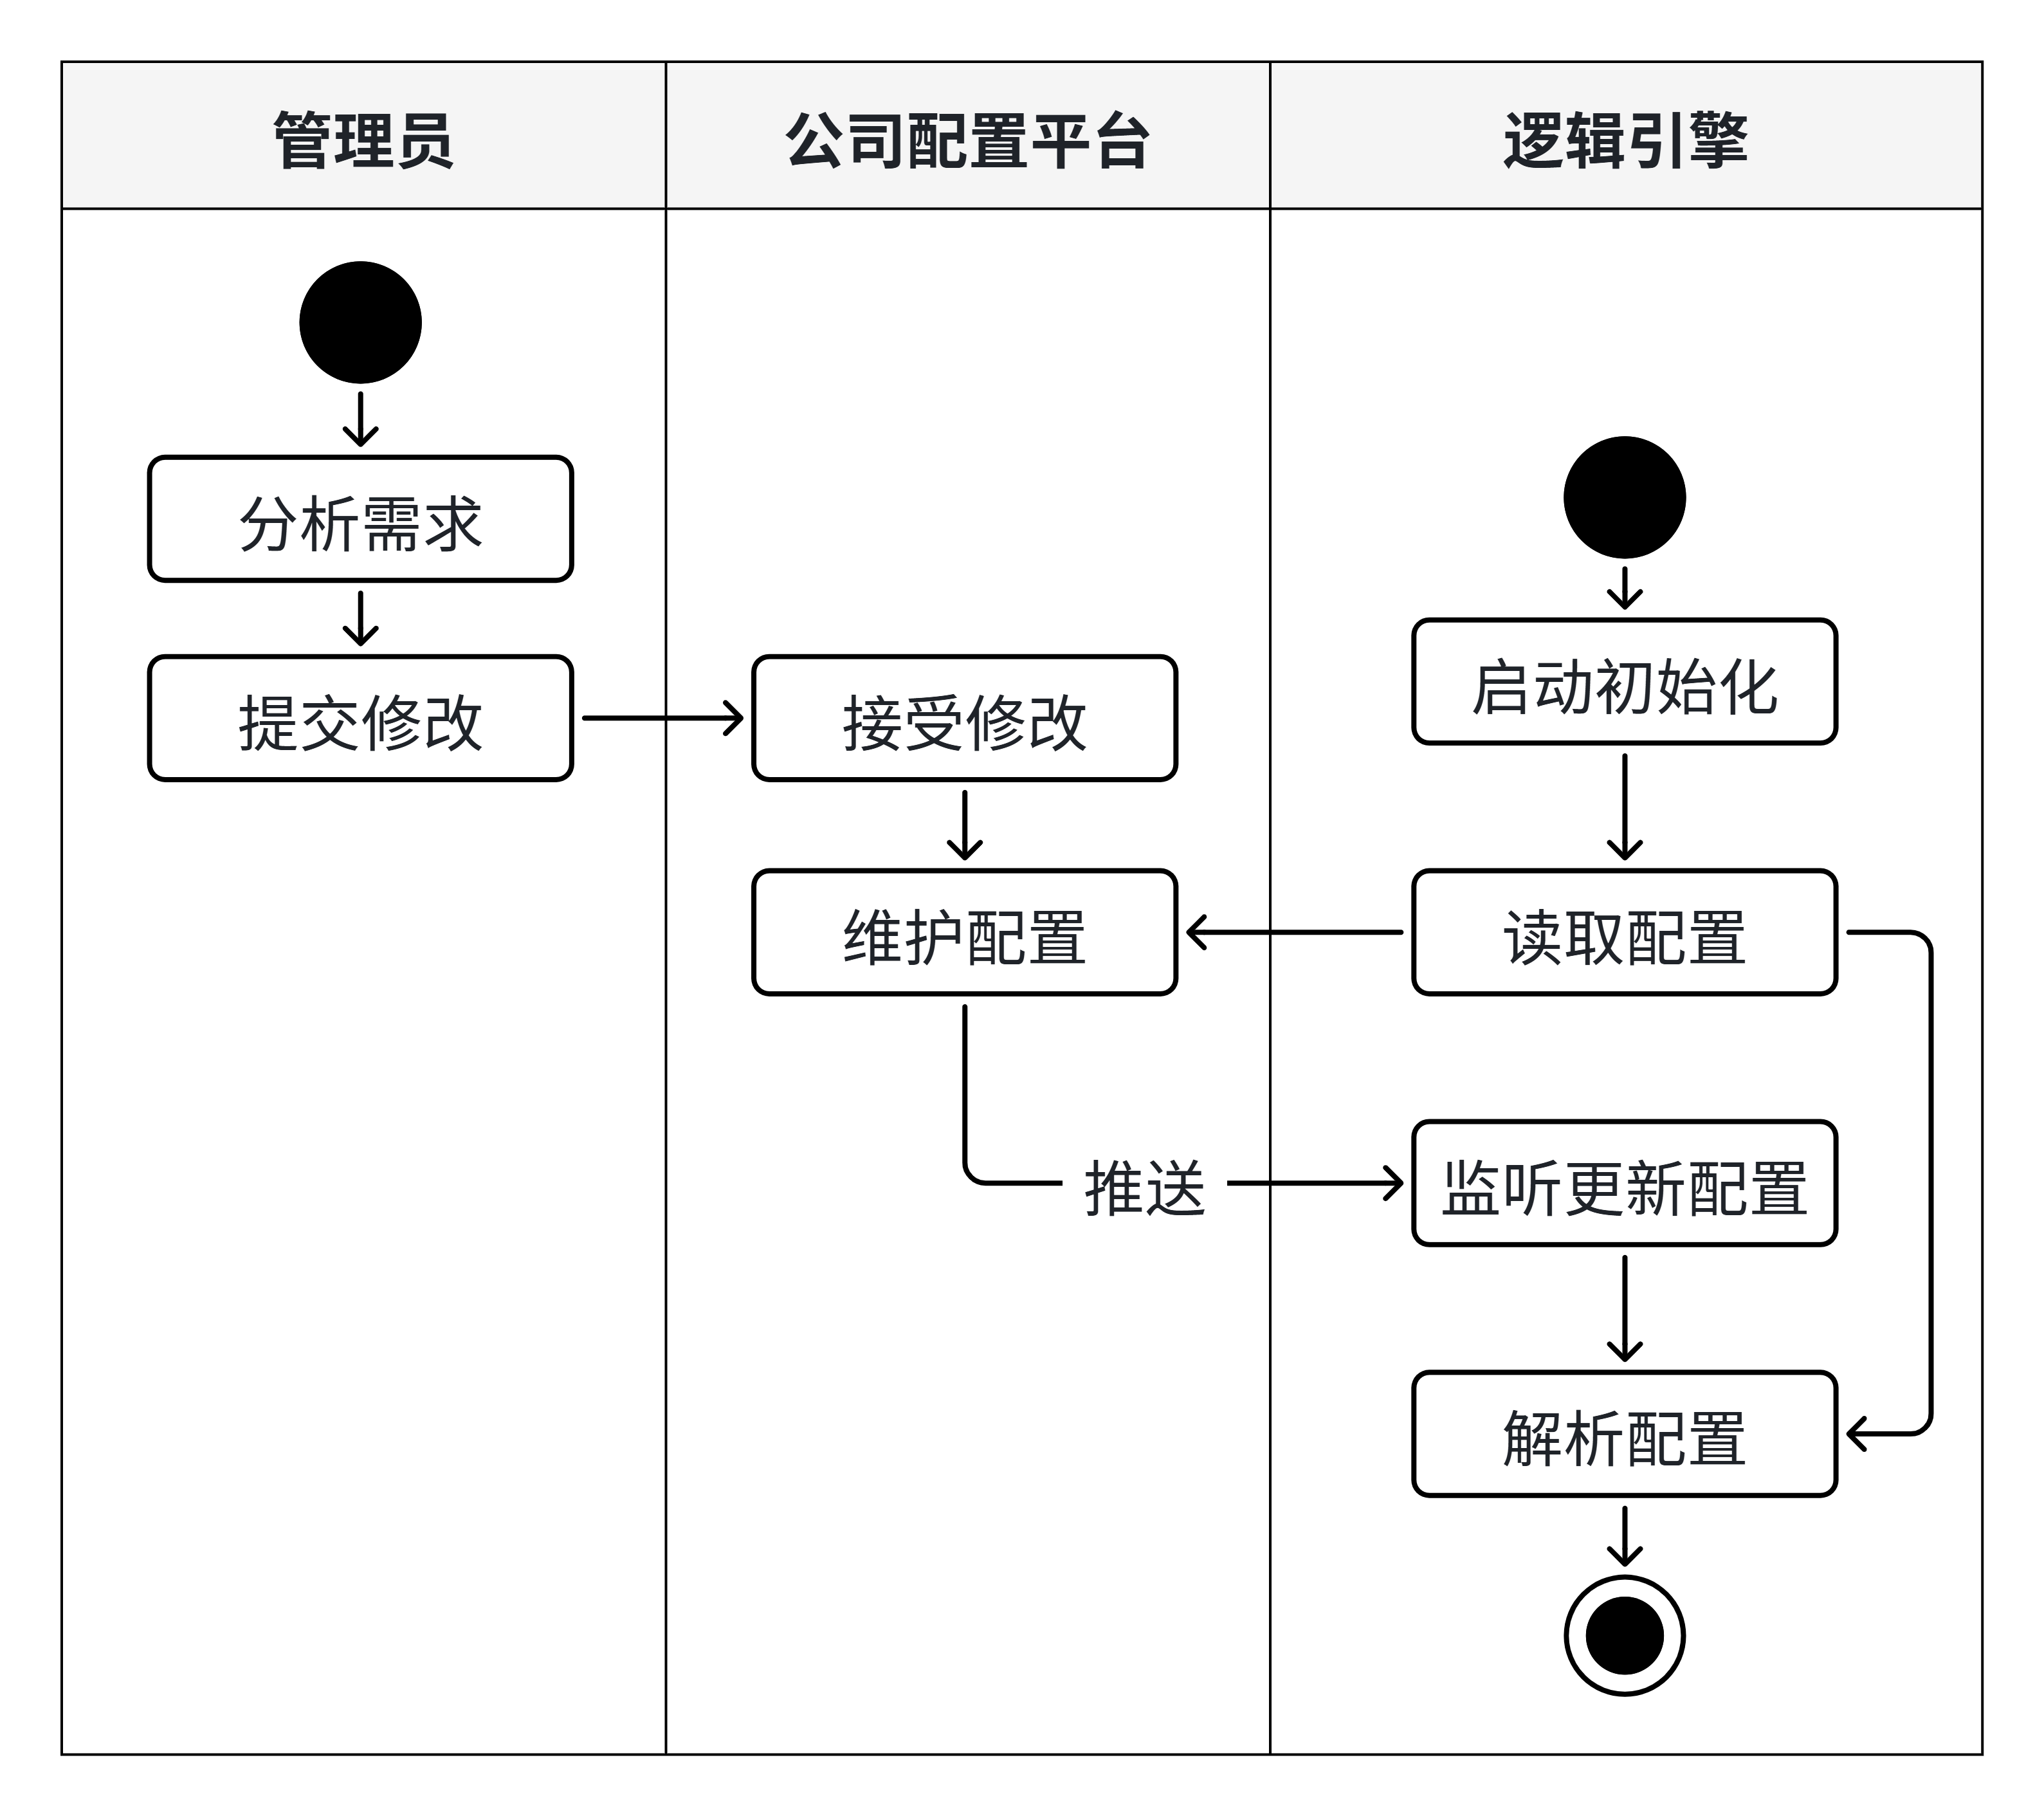
\includegraphics[width=0.8\linewidth]{figures/4/规则配置流程图.png}
    \caption{规则配置泳道图}
    \label{fig:enter-label}
\end{figure}

规则配置流程如图4.5所示。系统通过管理员在公司配置平台的策略修订实现逻辑规则的动态演进。平台接收修改请求并完成维护后，通过推送机制与逻辑引擎实现同步。逻辑引擎在启动初始化阶段完成既有配置的读取，并在运行期通过持续监听机制捕获动态更新指令，确保能够即时解析最新的策略文件并映射为可执行逻辑。该机制保障了调度策略的灵活性，使得系统能依据实时负载（如系统负载阈值）或特定业务约束，精准调控AI任务的准入状态。

\subsection{资源可用性检测机制}

针对计算资源互斥导致的任务串行与算力空耗难题，系统构建了精细化的算子资源管控体系。AI任务的运行高度依赖底层计算资源，其中CPU与内存多采用操作系统的抢占式调度策略，而GPU等高性能算力资源在执行大模型推理或训练时，通常表现为强独占性的临界资源。若系统缺乏对临界资源的感知能力，导致多个任务并发竞争同一物理GPU节点，将不可避免地引发显存溢出、数据冲突或执行失败等问题。为解决这一瓶颈，本系统设计并引入了“临界资源表”及其配套的冲突分析逻辑：
\begin{enumerate}
    \item 资源状态跟踪：系统通过临界资源表实时维护任务与资源的动态映射关系，记录资源占用状态等详细信息。该表可关联并锁定多个异构资源标识，从而实现对全局算力占用情况的精准捕获。
    \item 并发冲突判定：调度引擎在任务下发前，会检索临界资源表以识别目标资源是否处于锁定状态。通过这种资源拓扑识别机制，系统能够精准区分“可并发任务”与“互斥任务”，从而打破传统模式下盲目串行执行的限制。
    \item 动态分配与释放：系统根据资源表的反馈进行决策，若检测到冲突则将任务延时调度，若资源空闲则即时锁定并分配。
\end{enumerate}

通过该机制，系统实现了对算力资源的闭环管理，在保障AI任务执行安全性的同时，显著提升了集群的并发吞吐量与资源周转效率。

\subsection{负载均衡及性能优化设计}

为应对任务量增长以及需求的不断膨胀，本系统采用了可灵活扩展执行器的结构设计。然而，受预算及设备类型的限制，不同执行器节点的计算能力存在差异，进而致使其执行能力参差不齐。

本系统设计了一套调度机制，能够合理地将任务分配至不同节点。其中，系统借鉴了C语言编写的高性能HTTP服务器NGINX中用于处理动态负载均衡的权重轮询（Weighted Round Robin）算法。该算法主要用于处理动态负载均衡部分主要负责操作服务器的权重数据和向目标服务器转发客户的请求。此部分是在upstream机制中的加权轮询算法的基础上优化得到的\cite{10}。基于此，本系统实现了一个简化的权重轮训机制。每台执行机都配置有由管理员设定的权重。任务调度器依据这些权重，将任务分配至各台执行机。在分配任务之前，调度器会首先查询执行机的状态。若某台执行机处于满载状态，调度器便会跳过该机器。倘若所有执行机均处于满载状态，调度器则会跳过此次任务，而被跳过的任务将会等待下一次调度。

\subsection{数据同步模块}

本系统多个模块独立部署在不同的计算机系统上，彼此间有通信和数据同步需求。HTTP接口层与任务调度器通过 “任务池” 的形式实现任务同步。接口层在对任务参数与运行环境进行初步处理后，会把任务信息写入单独部署的数据库。任务调度器（其部署位置可能与接口层在同一台机器，也可能不同）从该数据库中提取处于特定状态的任务，并在恰当的时机将这些任务发送至Celery的任务队列。与此同时，任务调度器还会定时从Celery的结果队列中获取正在执行任务的相关信息，将任务的进度或结果写入数据库，最终这些信息会展示在网页上。执行器使用Celery执行端来接收Redis任务队列数据库中的任务数据，并定期将任务的进度条信息写入Redis的结果队列数据库。系统选用Redis作为消息队列，以满足 “管理平台程序”与 “执行器集群”之间的数据互通需求。在本系统中，会运用Redis的两个数据库（DB Number），分别专门用于任务的发送与接收。Redis的核心逻辑基于单线程运行，这一特性使得即便无需考虑任何并发锁设计，本系统也能够有效地避免任务的重复发送与重复消费。此外，Redis借助TCP协议进行数据传输，这进一步保障了任务信息不会丢失。

\subsection{容错与恢复机制}

本系统采用微服务架构。在这种架构下，不同服务间可能因版本更新不及时，引发数据传输问题，例如出现参数类型混淆，像float与int类型被错误混用的情况。此外，部分参数由操作员手动输入，这可能导致拼写错误或格式不符等问题。鉴于上述情况，本系统的API接口层在处理任务参数时，会针对参数中常见的基本错误进行初步纠错。纠错主要体现在以下几方面：
\begin{enumerate}
	\item 参数类型：若参数类型错误，虽能正常传递至AI任务，却会致使AI任务在执行中途出现异常，进而造成损失。基于此，本系统会先对参数类型展开初步校验与转化。只有在实在无法完成转化的情况下，才会向操作员抛出异常。
	\item 拼写错误：操作员在指定任务的部分参数时，有可能出现拼写错误。比如在填写某些列表时，可能会混淆全角与半角的逗号分隔符。针对此类情况，本系统设置了相应的恢复机制。
	\item 选择错误：当操作员做出存在矛盾的选择（比如选择在非GPU集群上运行GPU任务）时，本系统会尝试进行修正。具体而言，系统会通过办公软件向操作员提交审批申请，待审批通过后，便会自动更正参数，并将任务发送出去。
\end{enumerate}

\section{任务执行层概要设计}

面对日益增长的AI计算吞吐量，任务执行层被设计为解耦、可水平扩展的分布式算力单元。针对AI异构数据适配性欠佳的痛点，本层重点强化了执行环境的数据感知识别与鲁棒性适配。其核心功能需求通过以下三个机制实现：

\begin{enumerate}
    \item 异构环境初始化与数据映射机制：针对AI任务强数据依赖的特征，本层在初始化阶段通过参数画像匹配，实现远程附件的并发拉取与异构数据路径的本地化重定向。该机制确保了复杂AI参数在分布式执行节点间的一致性，从执行端消解了由于环境差异导致的数据处理障碍。
    \item 全生命周期监控与动态干预机制：系统需实时捕获任务在底层算力平台的运行状态。为提升运维灵活性，该机制支持任务在运行期的撤销与参数在线编辑，确保当业务逻辑或资源分配发生变更时，能即时终止旧进程并释放临界资源。
    \item 结构化结果回收与异常捕获机制：执行层负责建立高可靠的结果上报链路，对任务产出的非结构化数据及执行异常进行自动化收集与分类。通过细粒度的监控指标反馈，为上层调度中枢的决策闭环与容错恢复提供精准的数据支撑。
\end{enumerate}

\subsection{参数传递约定}

由于本系统所有组件均采用Python语言开发，组件间的参数传递统一基于Python原生数据类型。任务的启动参数采用Python字典（dict）类型，该类型内部并未设定任何硬性的格式要求。操作员注册任务并上传任务代码时，需要一并注册任务参数类型。在此之后，当启动任务时，系统的前端操作面板会自动显示与响应数据格式对应的表单，方便操作员填写。任务执行模块首先会准备任务执行所需要的参数。深度学习算法具有较强的数据依赖性，需要大量标注数据和计算资源\cite{liang2025survey}，所以这个过程还会拉取远端资源至本地临时目录，方便任务程序读取。首先程序会检查任务是否依赖远端附件。若依赖，则会向公司的COS（对象存储服务）拉取对应文件，并暂存在本系统的目录中。随后，程序会更改参数中的文件路径为本地路径，再传入任务，供任务代码读取。

\begin{figure}[ht]
    \centering
    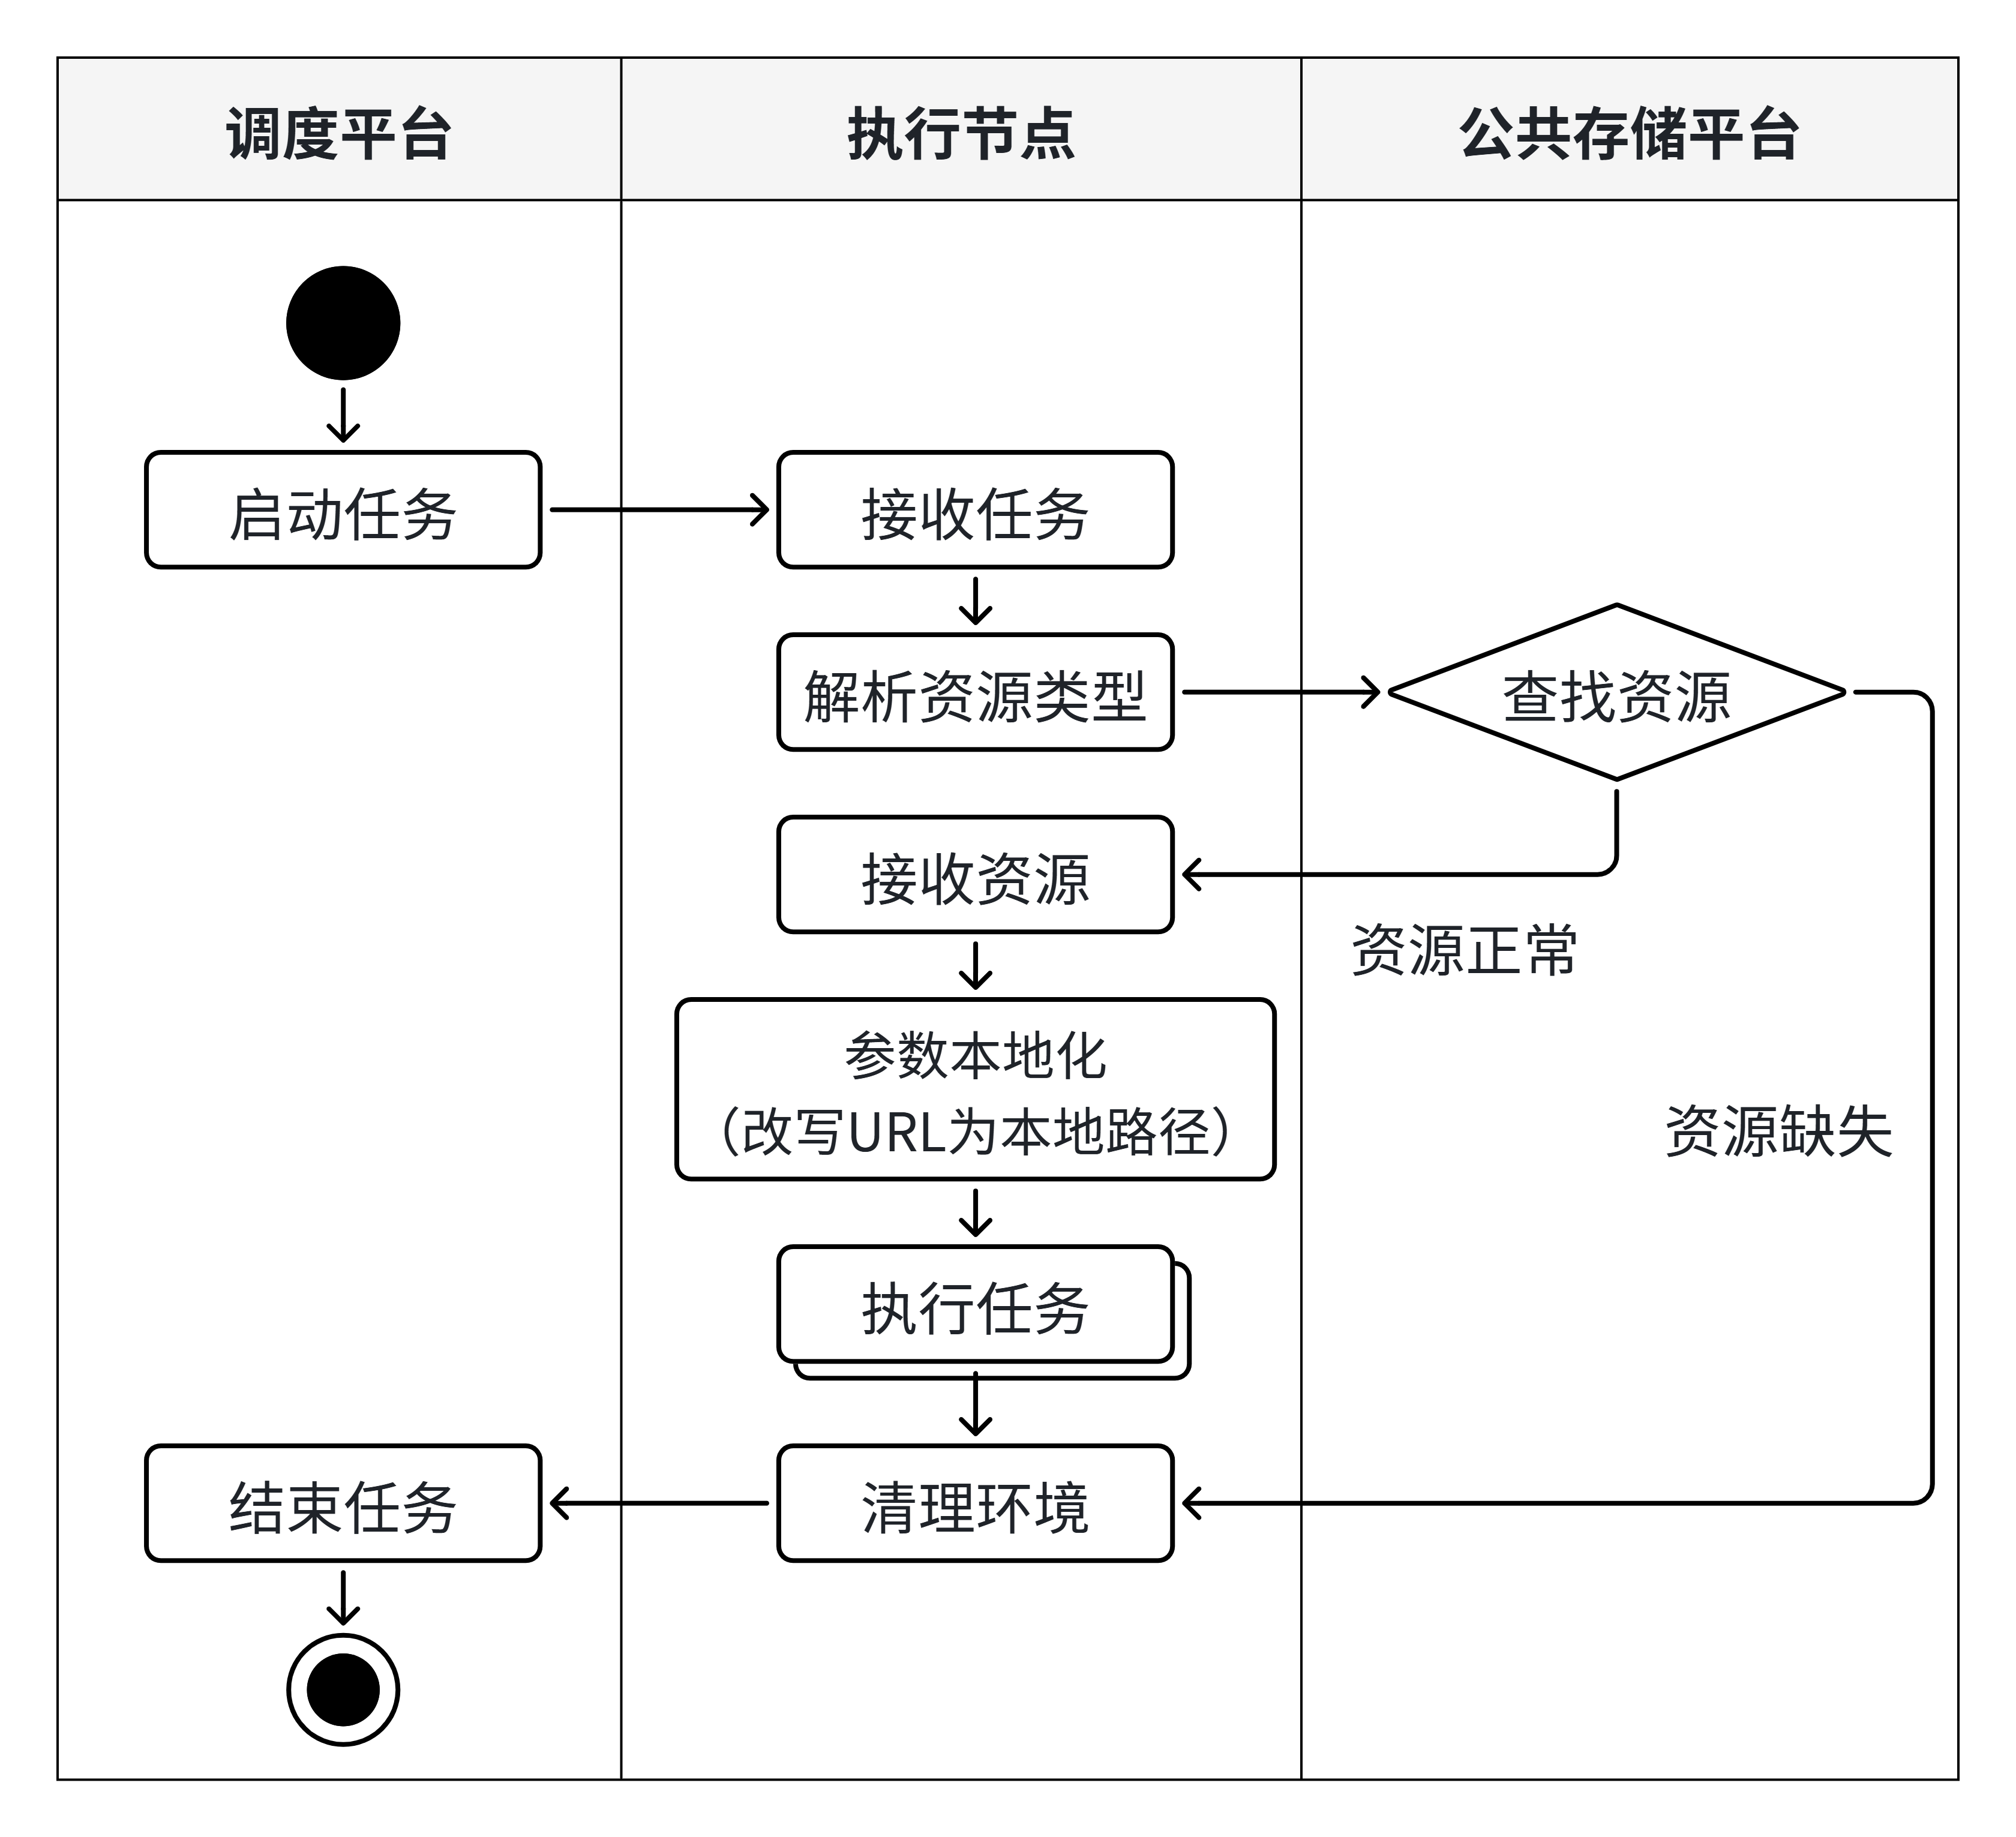
\includegraphics[width=0.8\linewidth]{figures/4/资源拉取流程图.png}
    \caption{资源拉取泳道图}
    \label{fig:enter-label}
\end{figure}

资源拉取流程如图4.6所示。

\subsection{任务编辑方式}

任务编辑机制为操作员提供了动态修正业务逻辑的途径，旨在解决因需求变动或录入失误导致的参数偏差。系统支持对处于任意生命周期阶段（等待或运行态）的任务进行在线编辑。执行编辑操作时，调度中枢首先检索任务状态：若任务正在运行，系统将立即终止其执行进程及相关子进程，从而强制释放其独占的GPU等临界资源，为后续并发调度腾出算力空间；若任务处于待发起状态，则直接进行逻辑覆盖。编辑完成后，原任务将被注销，系统依据修正后的异构参数生成新任务实例。由于参数变动可能引发新的资源互斥或策略约束，新任务将重新置于等待队列末尾，并联动自动化决策引擎重新进行准入判定。任务编辑流程如图4.7所示。

\begin{figure}[htbp]
    \centering
    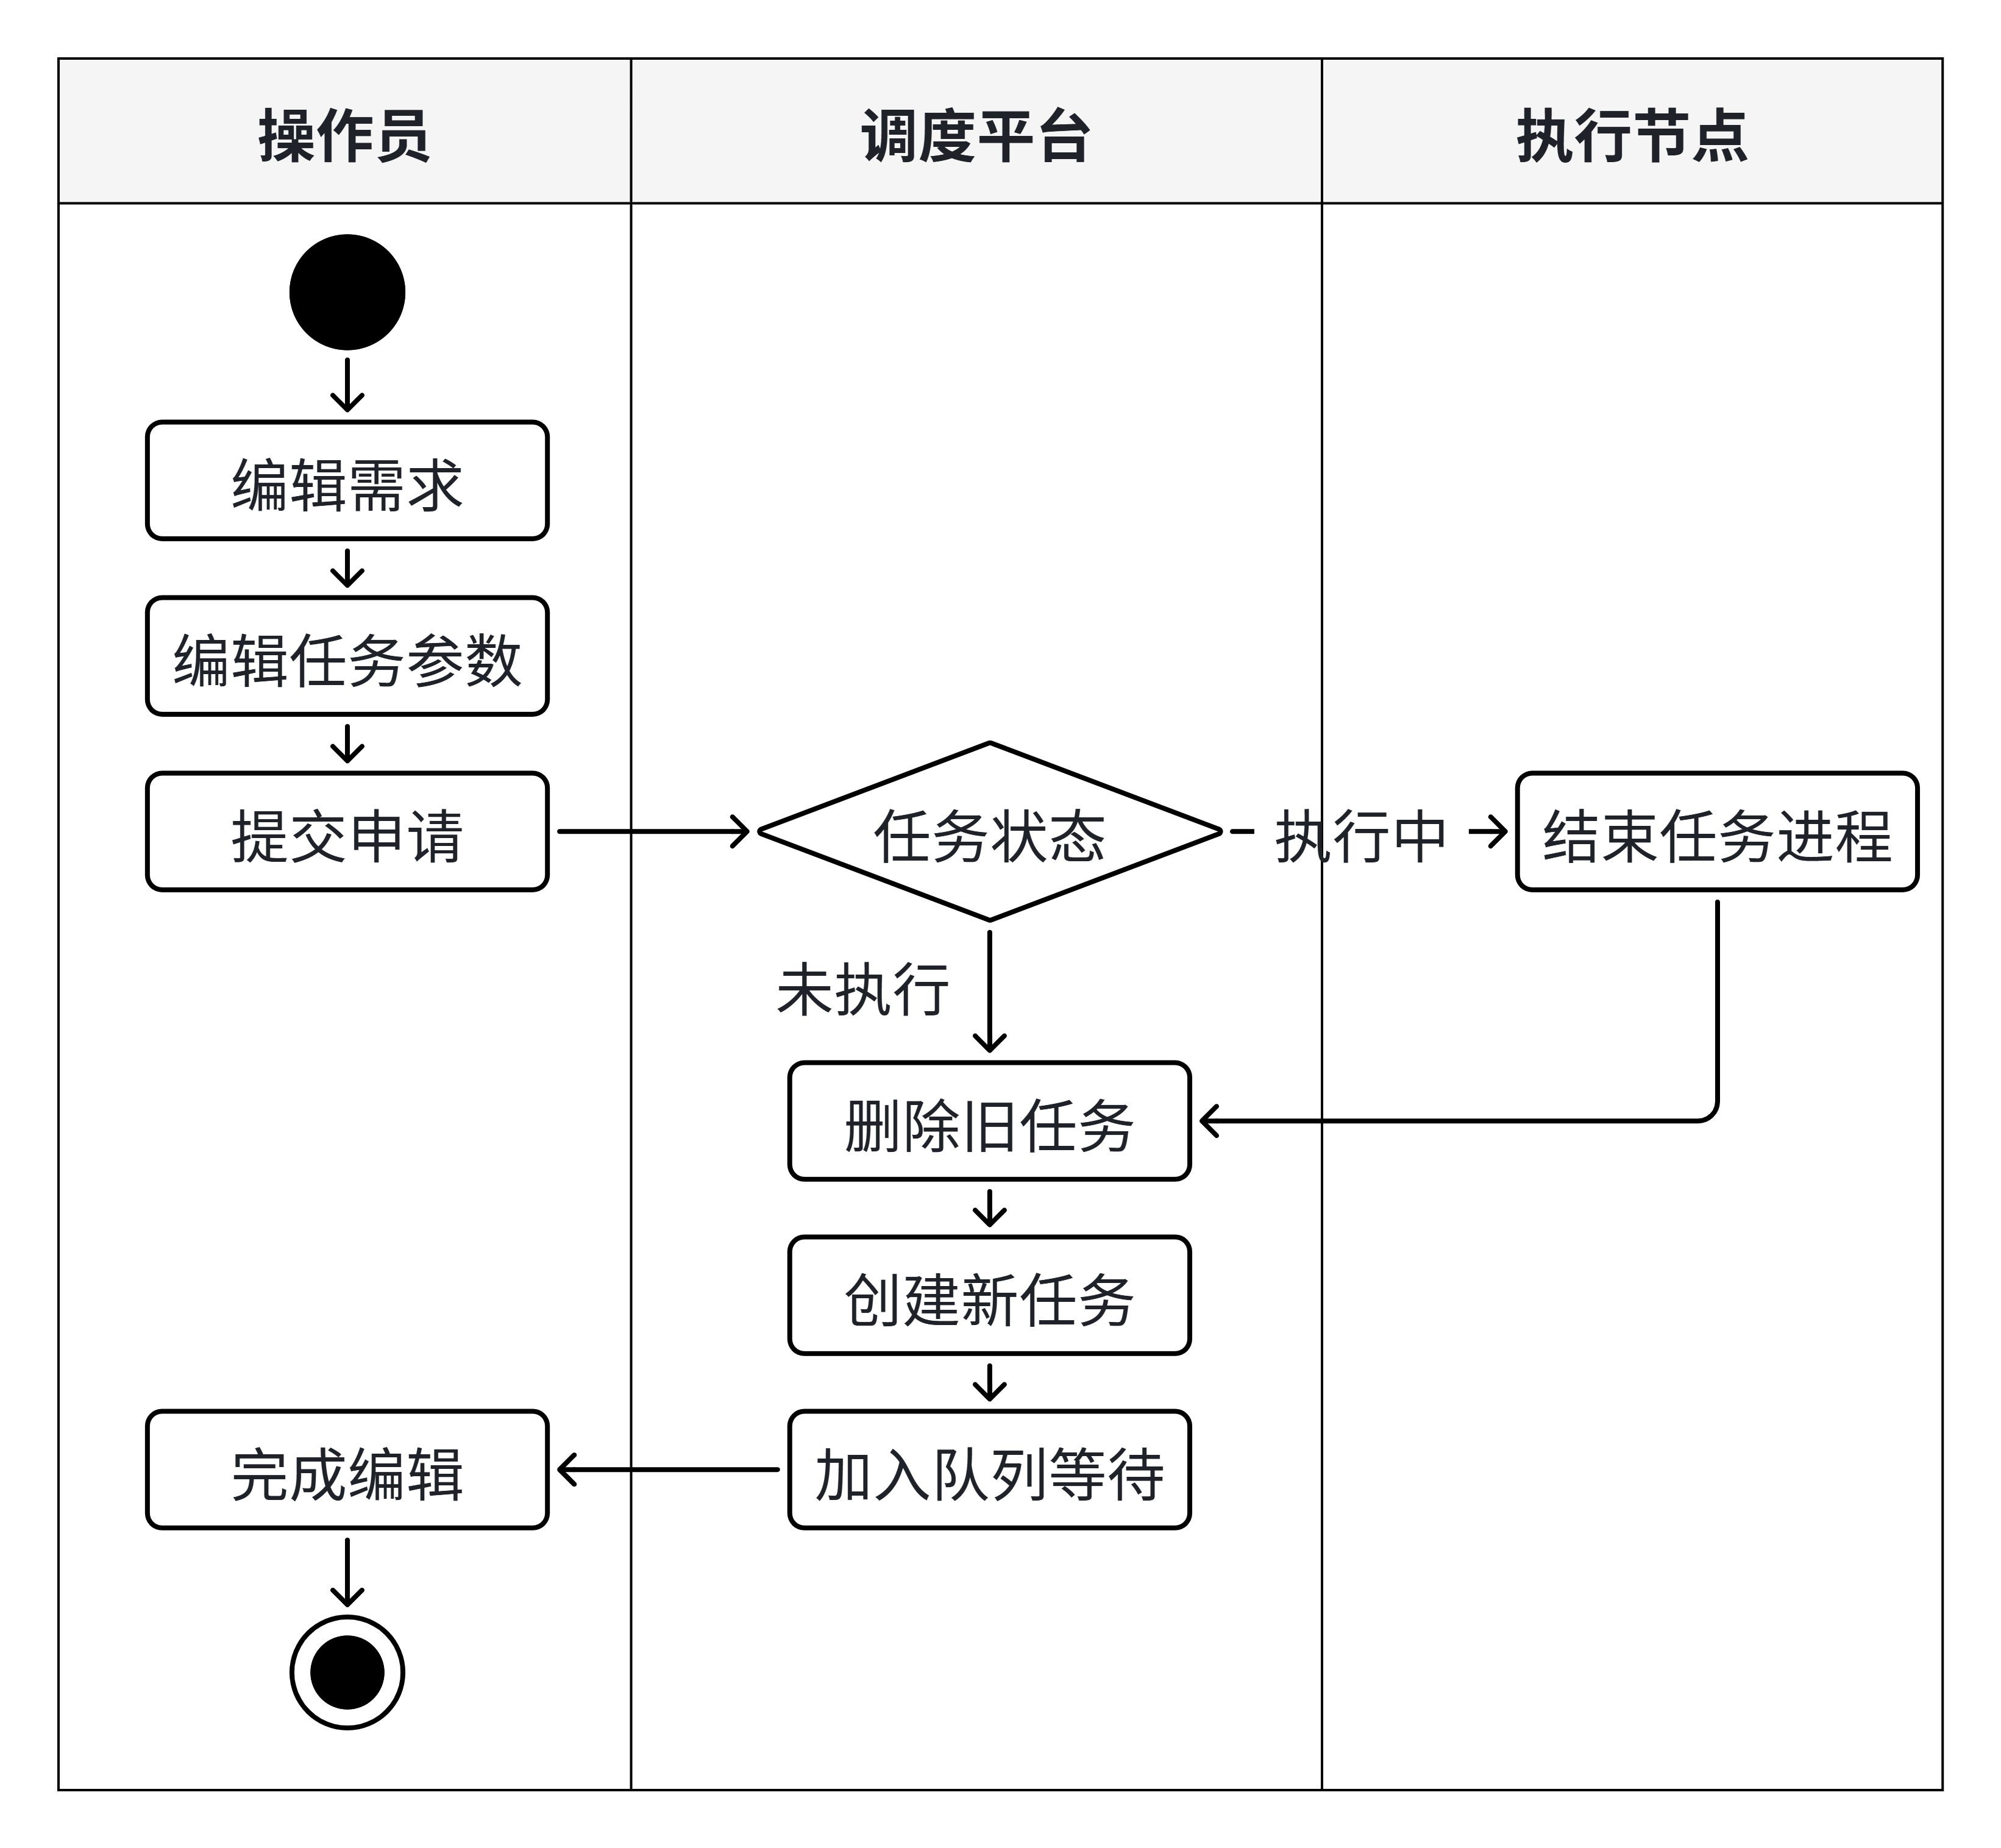
\includegraphics[width=0.9\linewidth]{figures/4/任务编辑流程.png}
    \caption{任务编辑泳道图}
    \label{fig:enter-label}
\end{figure}

任务撤销功能主要用于清理业务场景中不再需要的冗余任务，是优化系统算力周转率的重要手段。操作员可手动触发撤销指令，系统随后进入状态检查流程：对于执行中的任务，执行层将捕获撤销信号并强制关闭计算进程，即时阻断无效的算力消耗，解决资源浪费问题；对于处于等待队列的任务，系统则直接移除其元数据及关联的附件引用。撤销操作执行后，系统将从任务池中彻底剔除该实例的调度序列，并同步更新临界资源表，确保调度中枢能够基于最新的资源拓扑进行下一轮的智能并发分析。任务撤销流程如图4.8所示。

\begin{figure}[htbp]
    \centering
    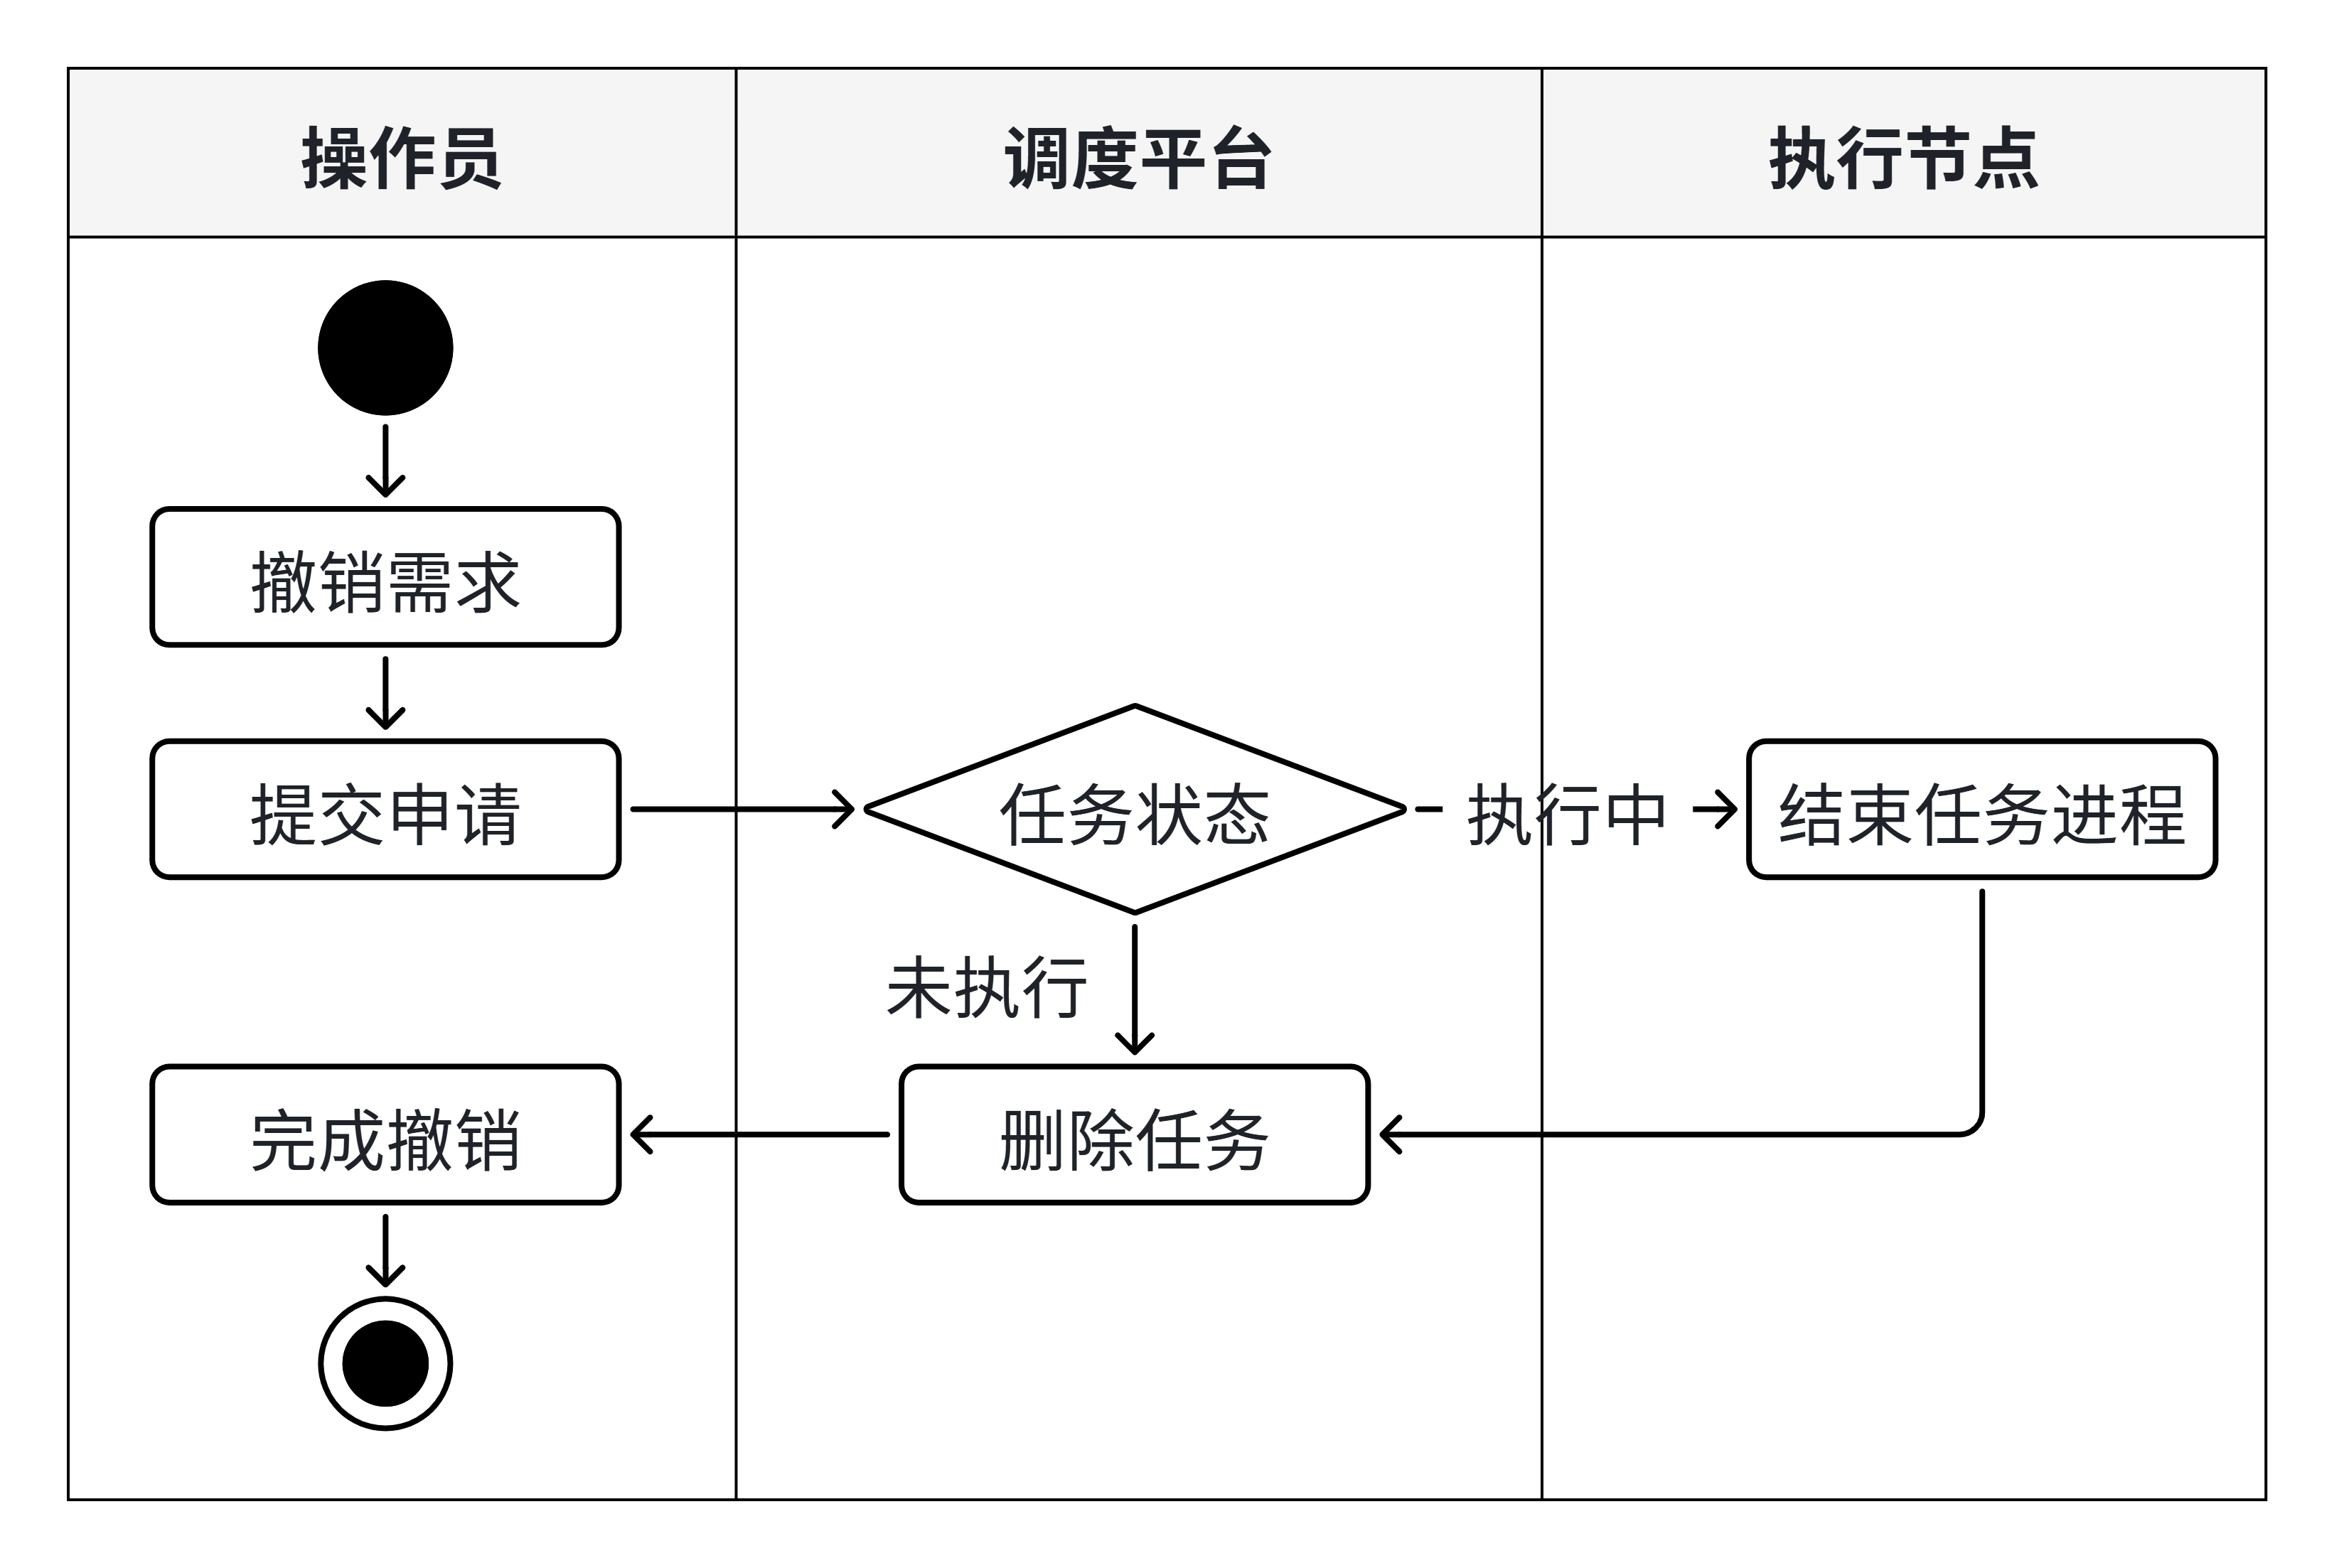
\includegraphics[width=0.9\linewidth]{figures/4/任务撤销流程.png}
    \caption{任务撤销泳道图}
    \label{fig:enter-label}
\end{figure}

\subsection{异常捕获机制}

本系统还需承接并处理任务执行过程中发生的异常情况。借助Python便捷的异常处理流程，本系统能够轻松识别任务运行时出现的错误。作为一种基于解释器的编程语言，它不会强制开发人员在开发过程中捕获异常\cite{s0218194022500814}，而AI任务的代码相对灵活，不安全的代码极有可能在没有经过全面的代码评审环节，就发布到平台上，因此极有可能在任务运行时抛出异常。本系统会捕获所有异常，并展开初步分析。倘若AI任务代码依照约定将具体异常日志打印到指定目录，本系统还能够整理这些日志，形成报表，并推送给操作员。异常发生后，所有中间文件和结果文件都会被上传，方便操作员自由下载，进而查看异常发生的原因。

\section{数据库表设计}

\subsection{数据库实体关系设计}

本系统核心数据模型由五个实体组成：用户、任务组、任务、附件以及资源占用记录。各实体的属性定义如下：

\begin{enumerate}
    \item 用户实体：存储身份及权限基础信息，包括用户ID、名称、账号有效性、注册时间及角色属性。
    \item 任务组实体：作为权限管理与资源隔离的基本单位，包含ID、名称、创建者、创建/更新/删除时间及删除状态位。
    \item 任务实体：记录AI调度的核心业务数据，包含ID、名称、创建者、生命周期时间戳（创建/修改/完成时间）、当前状态及异构参数列表。
    \item 附件实体：管理云端存储文件元数据，包含ID、显示名、对象存储URL、上传时间、上传者及删除标识。
    \item 资源占用记录实体：辅助调度算法进行互斥判断，包含记录ID、关联任务ID、资源名称及失效状态。
\end{enumerate}

\begin{figure}[htbp]
    \centering
    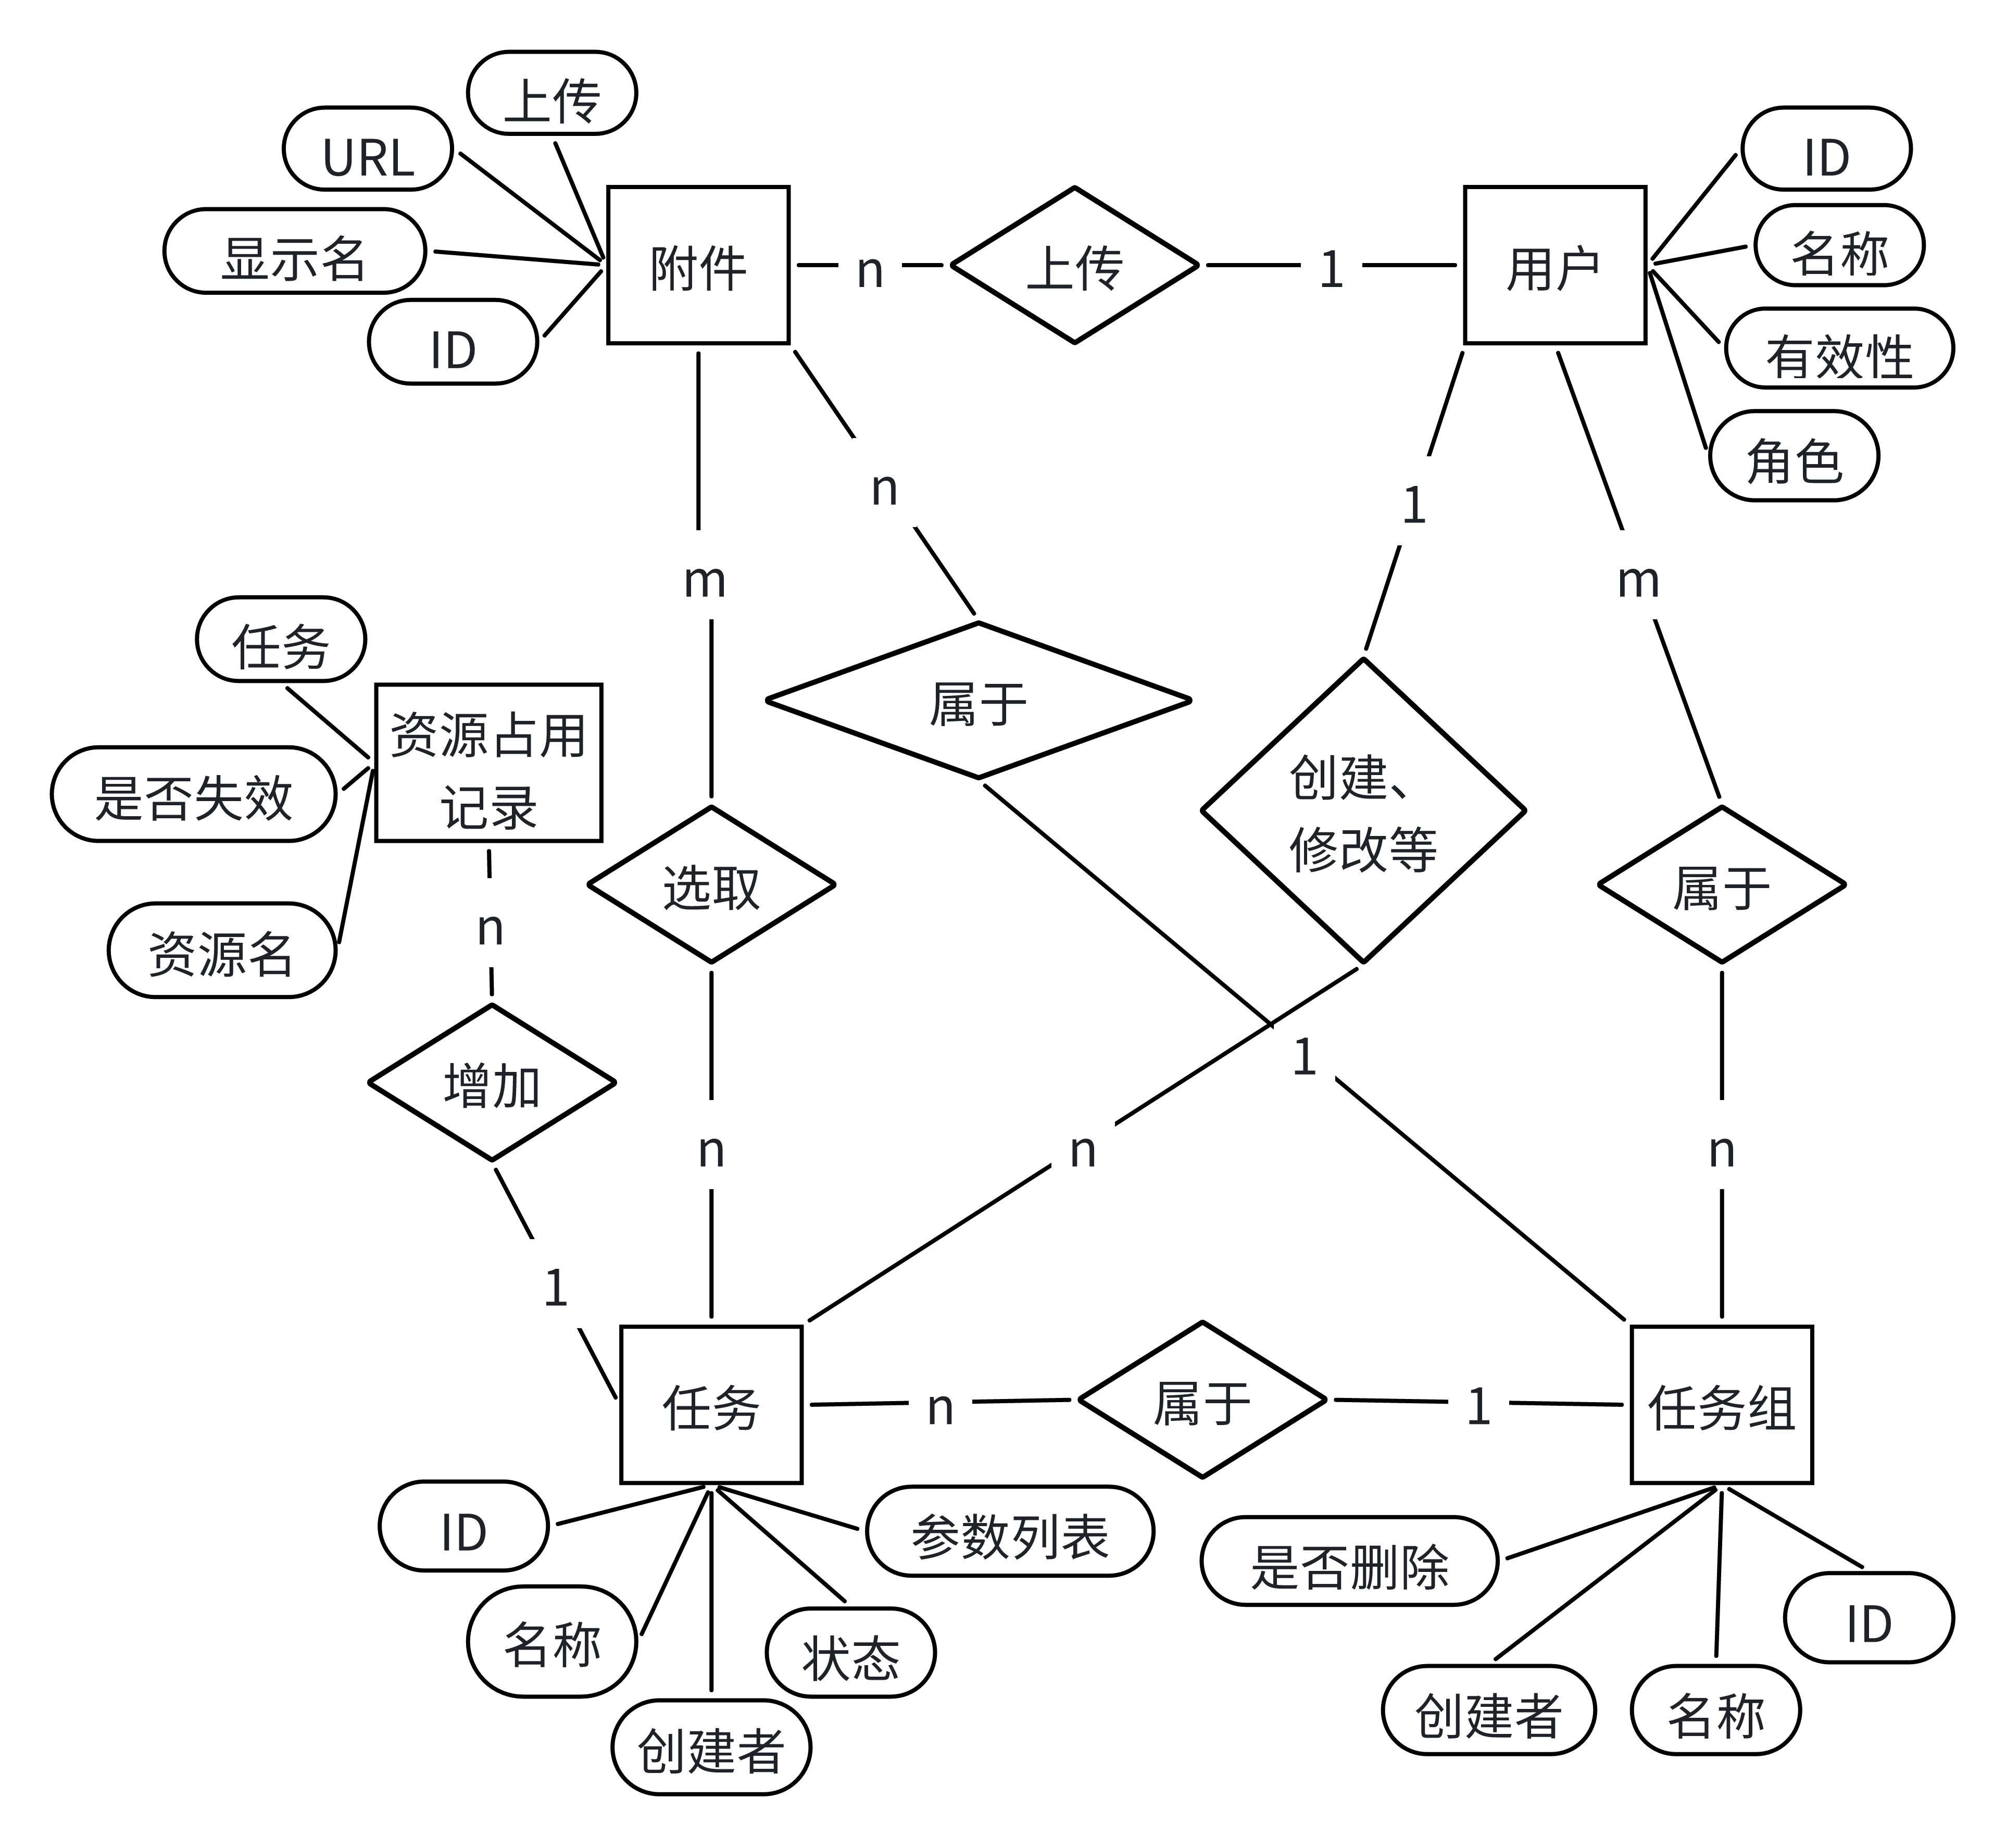
\includegraphics[width=\linewidth]{figures/4/数据库实体间关系.png}
    \caption{数据库实体间关系}
    \label{fig:enter-label}
\end{figure}

本系统的数据库实体关系如图4.9所示。

实体的相互关联逻辑梳理如下：

\begin{enumerate}
    \item 以“任务”为核心的关联逻辑。任务实体是系统逻辑的交汇点。用户与任务呈1:N关系，即一名用户可创建多个任务，但每个任务仅对应唯一创建者；任务组与任务呈1:N关系，确保任务在逻辑上归属于特定项目组以实现隔离。任务与附件呈M:N多对多关系，一个任务可选取多个预设附件，同一附件也可被不同任务重复引用。任务与资源占用记录呈1:N关系，用于精细化记录单个任务对多个临界资源的占用情况。
    \item 以“用户与权限”为核心的关联逻辑。用户是系统的操作主体。用户与任务组呈M:N关系，即用户可跨组协作，任务组也可包含多名成员，这种灵活的绑定关系支撑了系统的权限校验机制。此外，用户与附件呈1:N关系，明确了云文件的归属权。
    \item 以“隔离与调度”为核心的关联逻辑。任务组与附件呈1:N关系，实现了不同组间AI素材的逻辑隔离。资源占用记录主要服务于调度算法的互斥判断，通过与任务表的关联，协助调度器识别当前的算力冲突，保障多任务并发环境下的执行安全。
\end{enumerate}

本系统的类图如图4.10所示，该图将上述实体关系以类图的形式表达。

\begin{figure}[htbp]
    \centering
    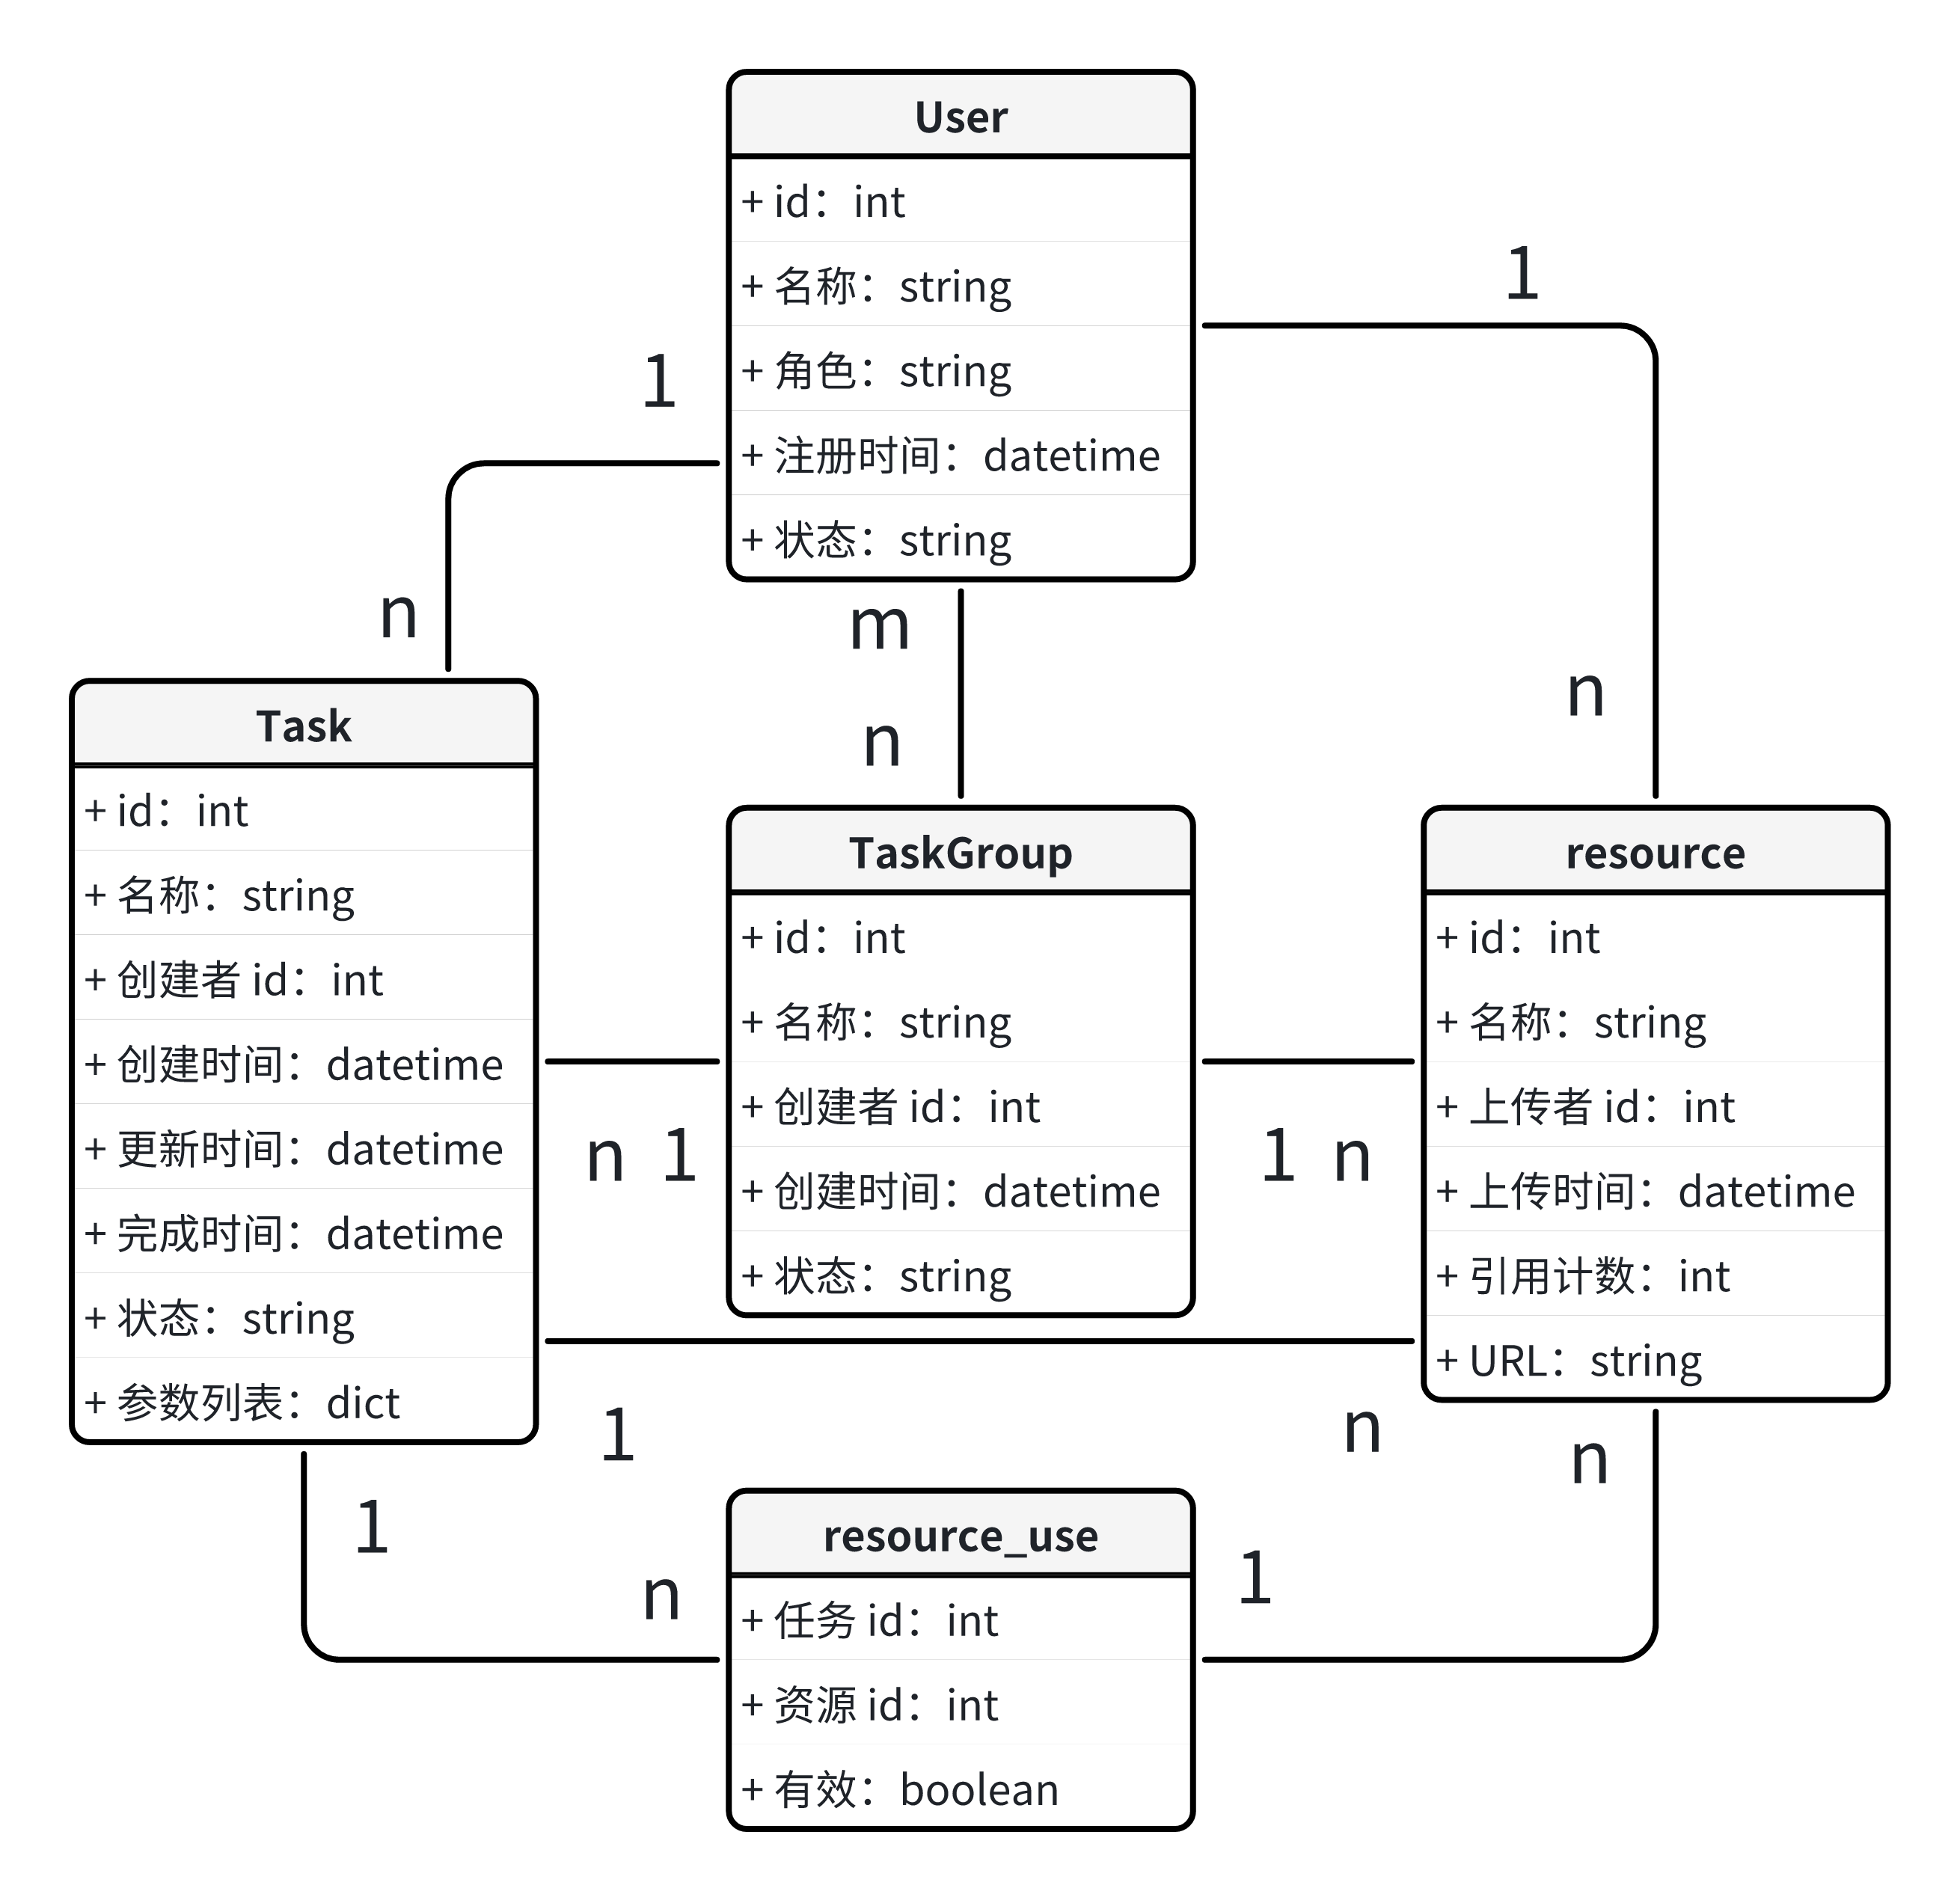
\includegraphics[width=\linewidth]{figures/4/本系统类图.png}
    \caption{本系统类图}
    \label{fig:enter-label}
\end{figure}

\subsection{数据库表设计}

本系统采用轻量级关系型数据库PostgreSQL进行数据持久化。根据实体功能及关联逻辑，将数据库表划分为基础权限类、核心业务类以及调度支撑类三个部分。

基础权限类表是构建整套调度系统安全底座的关键核心组件，在系统架构中主要承担着身份验证（Authentication）与访问控制（Access Control）的基础职能。该表的设计不仅能够严防非授权操作对高价值算力资源的非法侵占，更从技术维度确保了临界资源分配的审计合规性，为系统后续实现自动化准入决策与复杂的资源互斥分析提供了坚实且可信的操作上下文保障。

\begin{table}[htbp]
    \centering
    \caption{用户表}
    \begin{tabular}{llllll}
        \toprule
         序号 & 字段名 & 字段说明 & 类型 & 是否为空 & 说明 \\
         \midrule
            1 & id & 用户ID & int & N & PK\\
            2 & name & 用户名 & int & N & unique\\
            3 & valid & 账号是否有效 & boolean & N & \\
            4 & is\_delete & 是否已被删除 & boolean & N & \\
            5 & create\_time & 创建时间 & datetime & N & \\
            6 & update\_time & 资料更新时间 & datetime & N & \\
            7 & delete\_time & 删除时间 & datetime & N & \\
            8 & avatar & 头像链接 & varchar(200) & N & \\
         \bottomrule
    \end{tabular}
    \label{tab:my_label}
\end{table}

用户表如表4.1所示，该表用于存储操作员的核心属性及状态。在AI多任务调度流程中，系统需依托该表校验操作者的身份合法性，并为其分配相应的管理角色。表内设计的valid与is\_delete双重标识位，确保了在人员变动或账号注销时，系统能实现平滑的权限回收，保障安全。

\begin{table}[htbp]
    \centering
    \caption{任务组表}
    \begin{tabular}{llllll}
        \toprule
        序号 & 字段名 & 字段说明 & 类型 & 是否为空 & 说明 \\
        \midrule
1 & id & 任务组ID & int & N & PK \\
2 & name & 任务组名称 & int & N & unique \\
3 & owner & 任务组创建者 & varchar(200) & N &  \\
4 & is\_delete & 是否已被删除 & boolean & N &  \\
5 & create\_time & 创建时间 & datetime & N &  \\
6 & update\_time & 更新时间 & datetime & N &  \\
7 & delete\_time & 删除时间 & datetime & N &  \\
        \bottomrule
    \end{tabular}
    \label{tab:my_label}
\end{table}

任务组表如表4.2所示，该表是实现多租户隔离与资源归属管理的核心工具。针对大模型研发中不同业务团队共用底层集群的现状，任务组通过逻辑划分界定了任务与附件的所属权边界。这种设计不仅能有效规避跨组误操作引发的生产事故，还为后续针对特定业务线进行算力配额统计与审计提供了关键的元数据支撑。

核心业务类表作为系统架构中的逻辑基石，是支撑AI大模型异构数据深度适配、任务全生命周期精细化追踪以及复杂计算结果高可靠持久化的核心数据载体。针对当前主流调度方案在应对人工智能大模型任务时暴露出的适配性匮乏、非结构化参数校验门槛过高以及数据描述维度过于僵化等行业痛点，本系统立足于现代软件工程建模思想，在底层数据结构设计上实施了深度的范式优化。通过引入面向AI特性的Schema-less多维数据存储模型，并构建基于动态参数画像的关联机制，系统不仅能够敏锐感知并无缝兼容Prompt模板、采样超参数等高维度异构输入，更通过建立严密的任务状态机映射体系，实现了对调度指令从初始注入、排队挂起到最终结果回收的全流程数据闭环，从而为攻克AI多任务场景下的适配难题与调度瓶颈提供了稳固的数字化底座。

\begin{table}[htbp]
    \centering
    \caption{任务表}
    \begin{tabular}{llllll}
        \toprule
序号 & 字段名 & 字段说明 & 类型 & 是否为空 & 说明 \\
        \midrule
1 & id & 任务ID & int & N & PK \\
2 & name & 任务名称 & int & N & unique \\
3 & owner & 任务创建者 & varchar(200) & N &  \\
4 & kind & 任务类型 & varchar(200) & N &  \\
5 & is\_delete & 是否已被删除 & boolean & N &  \\
6 & update\_time & 更新时间 & dateTime & N &  \\
7 & datafiles & 数据文件列表 & varchar(1000) & Y &  \\
8 & queue\_task\_id & 在任务队列中的id & varchar(200) & Y &  \\
9 & progress & 任务进度 & JSON & Y &  \\
10 & result & 任务结果 & JSON & Y &  \\
11 & params & 任务启动参数 & JSON & Y &  \\
        \bottomrule
    \end{tabular}
    \label{tab:my_label}
\end{table}

任务表如表4.3所示，该表是调度指令的核心。为应对AI大模型任务中Prompt模板、采样参数以及模型超参数的异构性，系统采用JSON格式设计了params字段。这种Schema-less的设计能够灵活存储大模型任务的异构参数画像，有效解决了传统结构化表难以适配多样化AI任务的问题。此外，queue\_task\_id实现了业务逻辑层与底层Celery分布式队列的解耦关联，与之配套的 progress 与 result 字段采用JSON 类型，旨在构建一套完整的任务全生命周期观测体系。其中，progress 字段不局限于记录单一的百分比进度，更支持动态存储中间推理步骤、分段耗时等时序快照；而 result 字段则负责封装复杂的推理产出，包括但不限于文本响应、分词权重或多模态元数据。

\begin{table}[htbp]
    \centering
    \caption{附件表}
    \begin{tabular}{llllll}
        \toprule
        序号 & 字段名 & 字段说明 & 类型 & 是否为空 & 说明 \\
        \midrule
1 & id & 附件ID & int & N & PK \\
2 & name & 附件名称 & int & N & unique \\
3 & owner & 附件创建者 & varchar(200) & N &  \\
4 & is\_delete & 是否已被删除 & boolean & N &  \\
5 & update\_time & 更新时间 & dateTime & N &  \\
6 & url & 下载链接 & varchar(200) & N &  \\
7 & status & 数据集状态 & int & N &  \\
8 & count & 数据集大小 & int & N &  \\
9 & ref & 引用数 & int & N &  \\
        \bottomrule
    \end{tabular}
    \label{tab:my_label}
\end{table}

附件表如表4.4所示，该表专门用于管理大模型任务涉及的海量训练素材、验证数据集以及模型权重文件。由于AI任务具备强数据依赖的特征，附件表通过url字段对接公司对象存储服务，并利用status与count字段实现对异构素材的即时索引与量化评估。值得注意的是，表中设计的引用计数机制（ref）能够实时监测附件被不同任务调用的频率，为系统后续的存储空间自动回收与冗余清理提供了决策依据，从而在保障数据快速拉取的同时，最大化存储资源的利用率。

调度支撑类表是实现针对GPU等稀缺算力资源进行互斥识别与并发优化的关键数据底座。由于AI大模型任务在执行过程中对底层硬件具有显著的强排他性特征，若调度层缺乏对资源状态的实时感知能力，往往只能采取保守的串行策略，从而造成严重的算力资源浪费。

\begin{table}[htbp]
    \centering
    \caption{资源占用表}
    \begin{tabular}{llllll}
        \toprule
        序号 & 字段名 & 字段说明 & 类型 & 是否为空 & 说明 \\
        \midrule
1 & id & 记录ID & int & N & PK \\
2 & task\_id & 任务ID & int & N &  \\
3 & resource\_name & 资源名称 & varchar(200) & N &  \\
4 & is\_delete & 记录是否已被删除 & boolean & N &  \\
5 & create\_time & 占用记录创建时间 & datetime & N &  \\
6 & delete\_time & 删除时间 & dateTime & N &  \\
        \bottomrule
    \end{tabular}
    \label{tab:my_label}
\end{table}

资源占用表如表4.5所示，该表在系统中充当了全局“算力锁中心”的职能。通过动态记录task\_id与具体resource\_name（如特定的GPU编号或显存单元）的映射关系，系统能够以细粒度的方式实时追踪各临界资源的独占状态。在调度决策阶段，调度引擎通过检索该表执行资源互斥智能分析算法：若目标资源处于锁定状态且记录有效，则任务进入挂起队列；若资源空闲，则即时写入占用记录。表中的is\_delete与delete\_time字段配合执行层的异常捕获机制，实现了算力资源的即时释放与状态回收回滚。这一设计从底层数据结构上打破了调度流程的“黑盒”状态，为实现由传统串行执行向高效并发调度的转型提供了核心决策依据。

\section{本章小结}

本章初步介绍了系统的模块、子模块，以及数据库关系和表结构。在第一小节里，阐述了本系统的设计原则。基于上一章提出的几个方向性需求，此部分做出原则性规划，为系统设计明确总体方向与准则；第二小节对本系统的整体结构展开介绍，使读者初步认识系统的几大模块，构建起对系统架构的宏观印象；第三小节聚焦网络接入层，简要介绍了该层的权限鉴定和数据校验功能，这两个功能是保障网络接入安全与数据准确性的关键；第四小节介绍任务调度层。一方面对任务、资源可用性检测的自研算法予以说明，展现系统在任务与资源管理方面的独特方法，另一方面介绍负载均衡、数据同步、容错与恢复机制，这些机制确保任务调度的高效与稳定；第五小节谈及相对简单的任务执行层，主要介绍了附件和参数的初步处理、任务撤销与编辑，以及任务异常捕获机制，它们是任务顺利执行的重要保障；第六小节讲解本系统的数据库设计，主要涉及数据库实体关系和数据库表结构，这是系统数据存储与管理的基础。

\makeatletter
\@openrightfalse
\makeatother